\documentclass{myreport}
% =============================================
% Part 0 Edit the info
% =============================================

\major{大数据管理与应用}
\name{李峥昊}
\title{CryptoKitties数据分析报告}
\stuid{2201111618}
\college{管理学院}
\date{\zhtoday}
\course{大数据技术基础}
\coverpic{red}
\subcoverpic{figure/share.png}
\addbibresource[location=local]{reference.bib}
% \zihao{-4}


\begin{document}
% =============================================
% Part 1 Header
% =============================================
\makecover

\section{引言:区块链和以太坊}
在现在的互联网的架构中,在进行交易时,由于我们需要一个平台来对信息进行整合并提供一定的担保,从而引发出了两个问题:一是信任问题,由于个人数据集中存储和管理在服务器上,由大型公司掌控,因此个人数据很容易被收集、分析和使用;并且由于大型公司控制了数据,从而它们有能力控制和监督网络上的内容。二是价值分配问题,互联网上有众多的使用者去分享他们的产品或服务,但是财富大多是由提供服务的公司积累的。以音乐行业为例,据调查数据显示,由于中间商多、价值链复杂、版权数据不透明,音乐创作者权益处于弱势地位, 目前基于互联网流音乐的版税分配中,一首歌的版税分给唱片公司、操作系统和互联网播放平台的比例分别为42\%、30\%、和20\%,而词、曲作者总共只能分到8\%\cite{mekcoclub2022}。

区块链(Block Chain)技术使用哈希指针代替普通指针,通过哈希函数的collision resistance和hiding两个性质使得区块链中的数据无法被篡改而不被发现。从而保证了数据的安全性和不可更改性。同时引入分布式记账和共识机制,使多台分散的主机共同维护一个网络。

以太坊(Ethereum)是区块链的一个应用。与比特币(Bitcoin)不同的是,以太坊通过一个状态树来记录所有有余额的用户数据,如余额、智能合约代码、存储数据等。通过交易树来记录以太坊网络上的所有交易信息,如交易的发起者、接受者、交易数据、费用等。通过收据树记录交易执行的结果信息,如交易是否执行成功、执行后的账户状态、智能合约产生的输出等。

此外,以太坊还支持智能合约的应用。智能合约是一种部署在区块链上的程序,用户通过调用智能合约以实现某些特定功能,并支付一定的gas作为调用计算资源的报酬。智能合约与前端界面共同构成了可供用户使用的去中心化应用(DApp,Distributed Application)。


\section{CryptoKitties及其智能合约}
\href{https://www.cryptokitties.co}{CryptoKitties}是一款部署在以太坊区块链上的DApp,是第一个大规模的以太坊DApp,在2017年发布后受到了广泛的关注。它允许用户生成、购买、销售和交换CryptoKitties,并且每只CryptoKitty都是一个独特的、不可复制的数字资产,具有一定的收藏价值。

CryptoKitties的智能合约地址为\href{https://etherscan.io/address/0x06012c8cf97bead5deae237070f9587f8e7a266d#code}{0x06012c8cf97BEaD5deAe237070F9587f8E7A266d},除了基因算法,其代码在以太坊上公开可见。CryptoKitties智能合约的结构如图\ref{fig:craptokitties contract}所示。
\begin{figure}[!htbp]
	\centering
	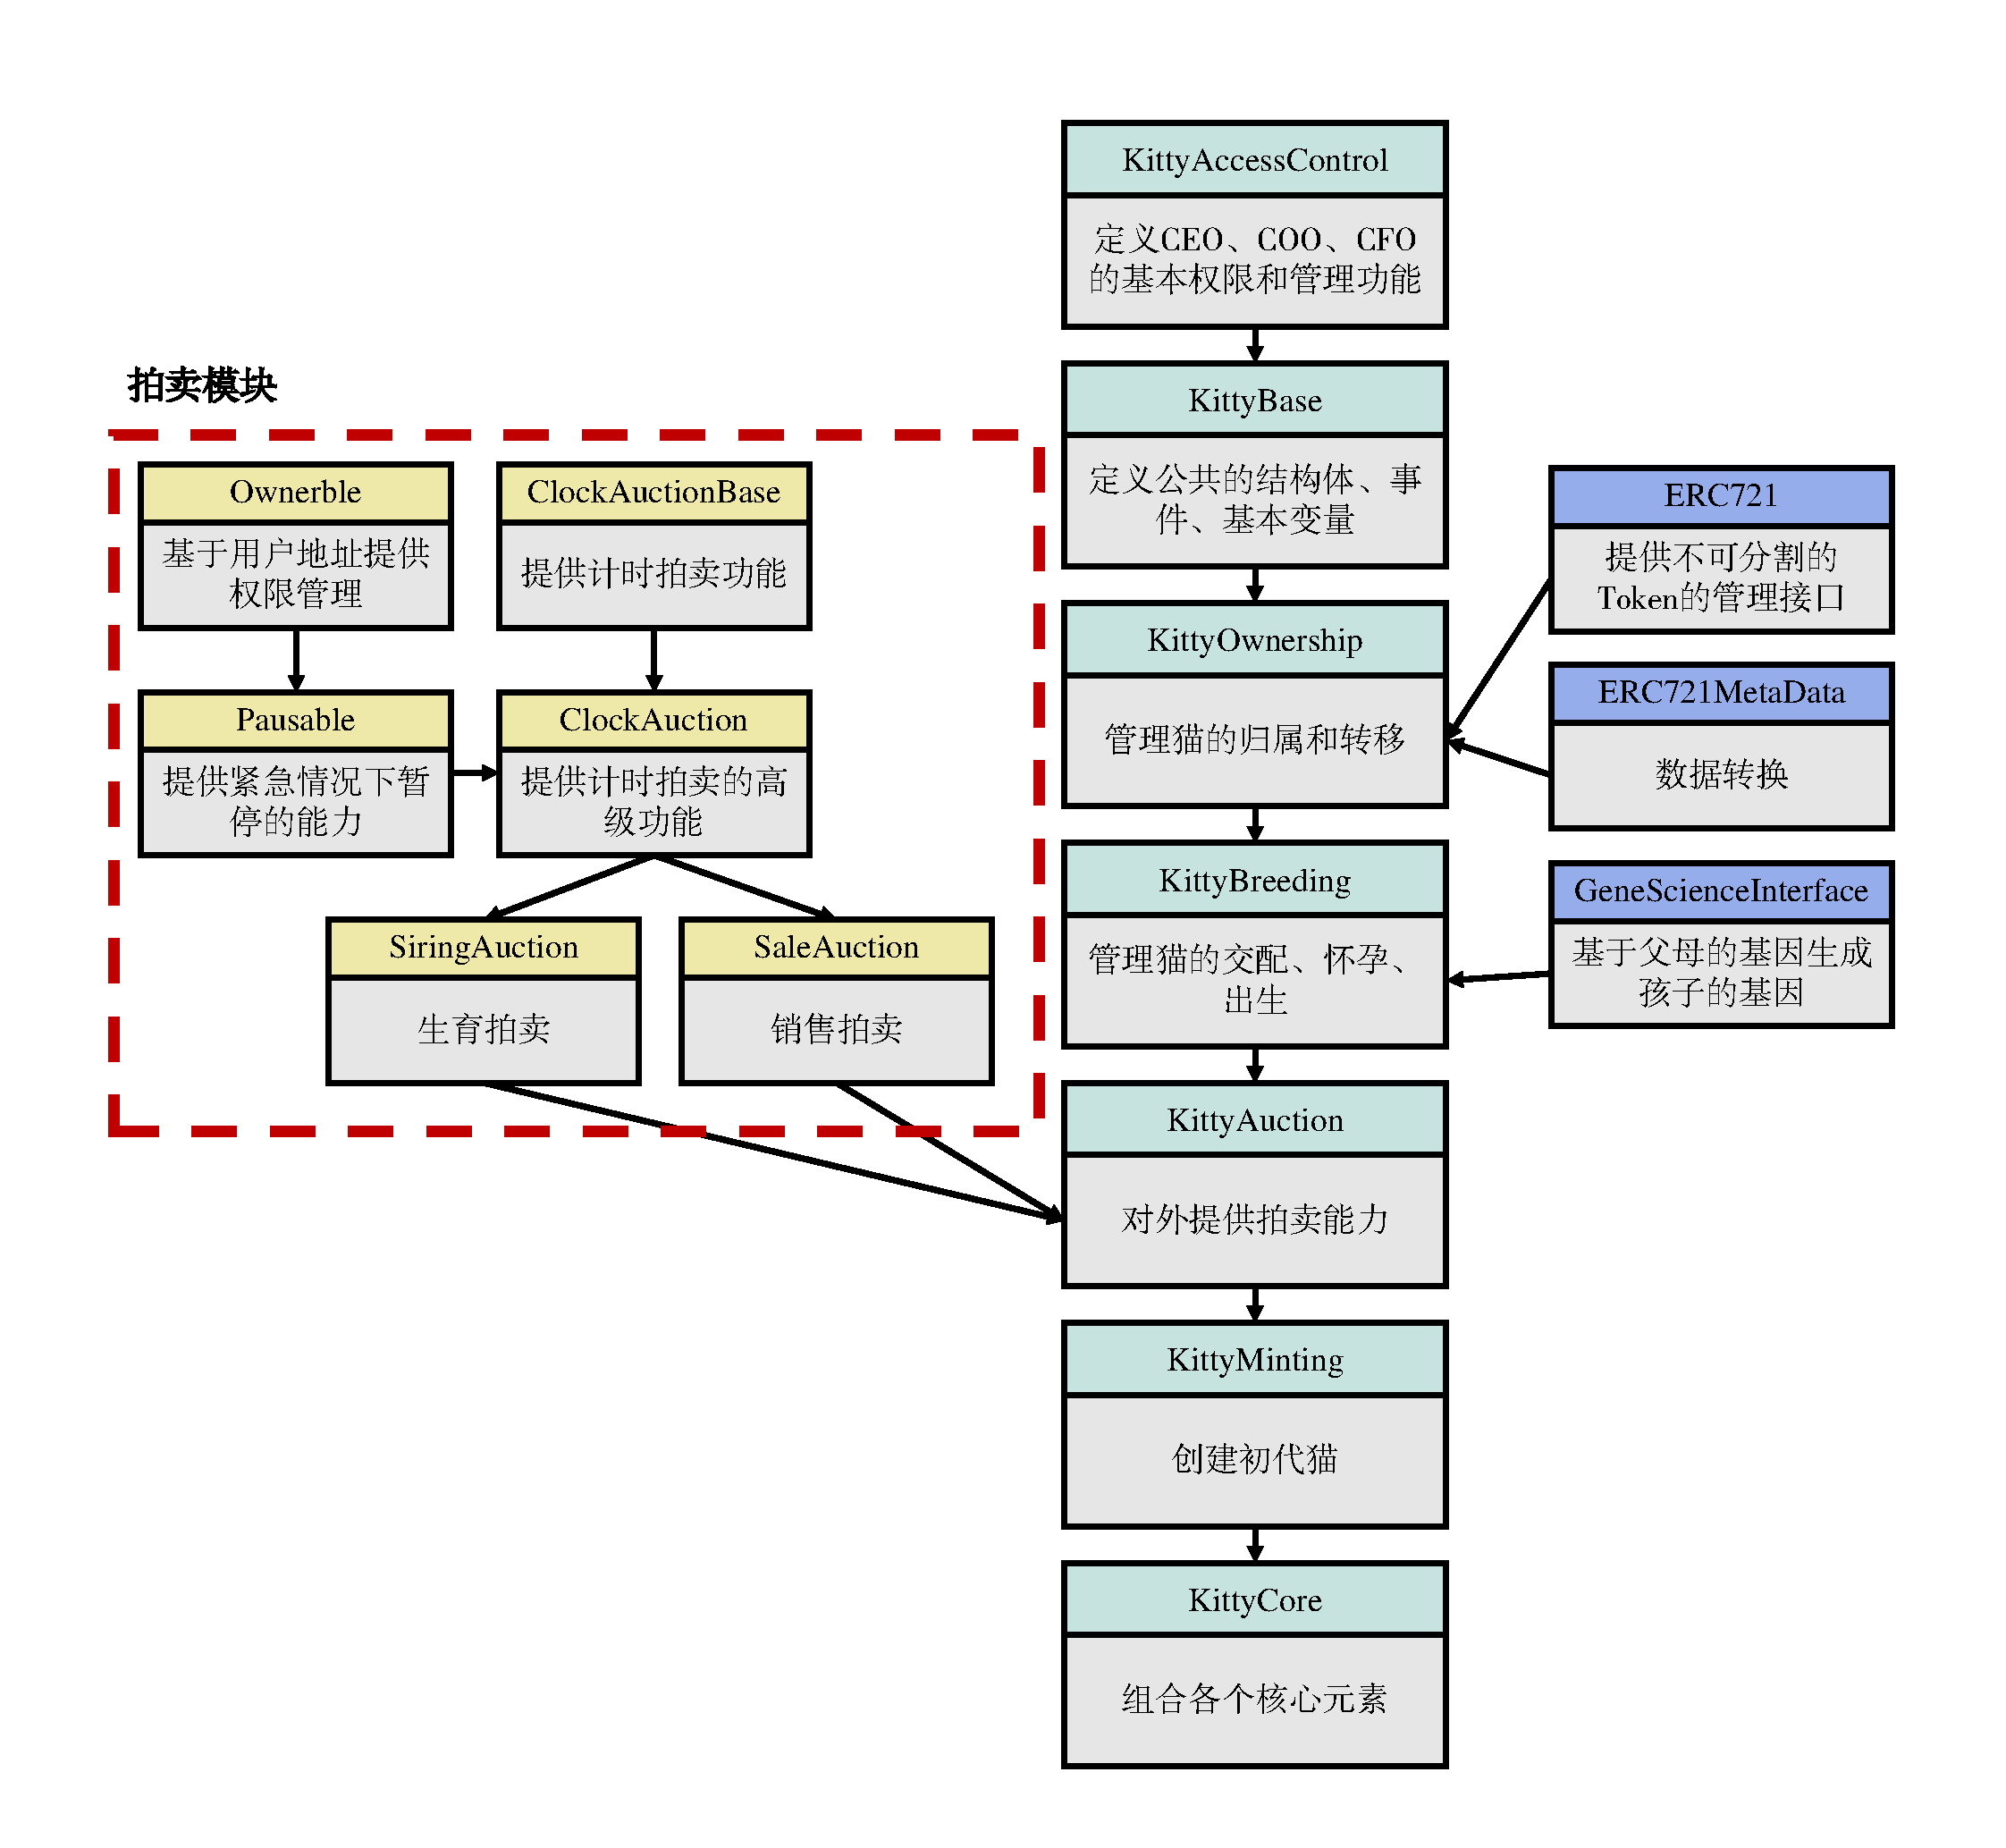
\includegraphics[width=\linewidth]{figure/cryptokitties.pdf}
	\caption{CryptoKitties智能合约的结构图}
	\label{fig:craptokitties contract}
\end{figure}

其中,以下几个函数所产生的数据比较重要。这些函数主要集中在三个合约地址,Core:\href{https://etherscan.io/address/0x06012c8cf97bead5deae237070f9587f8e7a266d}{0x0601\_266d}, Sale Auction:\href{https://etherscan.io/address/0xb1690c08e213a35ed9bab7b318de14420fb57d8c}{0xb169\_7d8c}和 Siring Auction:\href{https://etherscan.io/address/0xc7af99fe5513eb6710e6d5f44f9989da40f27f26}{0xc7af\_7f26}。为简短起见,仅保留地址的开头四位和结尾四位。函数具体信息如表\ref{tbl:function}所示。
\begin{enumerate}
\item createSaleAuction。创建一个计时拍卖,拍卖猫的所有权,价格随着时间线性变化。在用户成功创建拍卖后的同时,用户的猫将转移给CryptoKitties下的一个地址。用户可以随时无条件取消拍卖,取消拍卖时调用cancelAuction函数,将猫从CryptoKitties还给用户。
% createSaleAuction(uint256 _kittyId, uint256 _startingPrice, uint256 _endingPrice, uint256 _duration)
\item createSiringAuction。创建一个计时拍卖,拍卖猫的交配权,价格随着时间线性变化,用户可以随时无条件取消拍卖,取消拍卖时调用cancelAuction函数,将猫从CryptoKitties还给用户。如果交配成功,则卖方收回猫的所有权,买方猫怀孕并获得小猫的所有权。双方的猫共同进入休息期。
% createSiringAuction(uint256 _kittyId, uint256 _startingPrice, uint256 _endingPrice, uint256 _duration)
\item giveBirth。在交配以后,用户可以得到新的猫,其具体方式为:获取母亲和父亲的基因,通过基因算法(遗传和变异)来确定子代的基因,并得到新的小猫。在小猫出生后,将小猫的所有权移交给母亲的持有者上。
% giveBirth(uint256 _matronId)
\item breedWithAuto。用户可以繁衍自己的猫,即自己的猫和自己的猫交配。
%breedWithAuto(uint256 _matronId, uint256 _sireId)
\item transfer。用户可以将猫的所有权转移给另外一个人。
% transfer(address _to, uint256 _tokenId)

\item bidOnSiringAuction。用户可以对生育拍卖进行出价,竞拍成功后,用户获得一只已怀孕的猫,随后可以调用giveBirth获得新的小猫。
% bidOnSiringAuction(uint256 _sireId, uint256 _matronId)
\item bid。用户可以对销售拍卖进行出价,竞拍成功后获得这只猫的所有权。
% bid(uint256 _tokenId)
\end{enumerate}


\begin{table*}[!htbp]
	\centering
	\caption{CryptoKitties函数详情}
	\begin{tabular}{lcccc}
		\toprule
		name&contract&method&log&data\\
		\midrule
		\multirow{4}{*}{createSaleAuction}&\multirow{4}{*}{Core}&\multirow{4}{*}{0x3d7d3f5a}&\multirow{2}{*}{Transfer}&kittyId\\
		&&&&startingPrice\\
		&&&\multirow{2}{*}{AuctionCreated}&endingPrice\\
		&&&&duration\\

		\midrule
		\multirow{4}{*}{createSiringAuction}&\multirow{4}{*}{Core}&\multirow{4}{*}{0x4ad8c938}&\multirow{2}{*}{Transfer}&kittyId\\
		&&&&startingPrice\\
		&&&\multirow{2}{*}{AuctionCreated}&endingPrice\\
		&&&&duration\\

		\midrule
		\multirow{2}{*}{giveBirth}&\multirow{2}{*}{Core}&\multirow{2}{*}{0x88c2a0bf}&Birth&\multirow{2}{*}{matronId}\\
		&&&Transfer&\\

		\midrule
		\multirow{2}{*}{breedWithAuto}&\multirow{2}{*}{Core}&\multirow{2}{*}{0xf7d8c883}&\multirow{2}{*}{Pregnant}&matronId\\
		&&&&sireId\\

		\midrule
		\multirow{2}{*}{transfer}&\multirow{2}{*}{Core}&\multirow{2}{*}{0xa9059cbb}&\multirow{2}{*}{Transfer}&address\_to\\
		&&&&tokenId\\

		\midrule
		\multirow{4}{*}{bidOnSiringAuction}&\multirow{4}{*}{Core}&\multirow{4}{*}{0xed60ade6}&Gene&\multirow{2}{*}{sireId}\\
		&&&AuctionSuccessful&\\
		&&&Transfer&\multirow{2}{*}{matronId}\\
		&&&Pregnant&\\

		\midrule
		\multirow{2}{*}{bid}&\multirow{2}{*}{SaleAuction}&\multirow{2}{*}{0x454a2ab3}&AuctionSuccessful&\multirow{2}{*}{tokenId}\\
		&&&Transfer&\\

		\midrule
		\multirow{2}{*}{cancelAuction}&\multirow{2}{*}{SaleAuction}&\multirow{2}{*}{0x96b5a755}&AuctionCancelled&\multirow{2}{*}{tokenId}\\
		&&&Transfer&\\

		\midrule
		\multirow{2}{*}{cancelAuction}&\multirow{2}{*}{SiringAuction}&\multirow{2}{*}{0x96b5a755}&AuctionCancelled&\multirow{2}{*}{tokenId}\\
		&&&Transfer&\\



		\midrule
		\textbf{note: contract address}&&&&\\
		Core:&\multicolumn{4}{l}{0x06012c8cf97BEaD5deAe237070F9587f8E7A266d}\\
		SaleAuction:&\multicolumn{4}{l}{0xb1690C08E213a35Ed9bAb7B318DE14420FB57d8C}\\
		SiringAuction:&\multicolumn{4}{l}{0xC7af99Fe5513eB6710e6D5f44F9989dA40F27F26}\\
		\bottomrule
	\end{tabular}
	\label{tbl:function}
\end{table*}


\section{数据获取}

首先尝试从sql的CryptoKitties数据库中获取数据,其代码如listing~\ref{SQL:1}所示。图\ref{fig:saleauction count 1}中显示了saleAction函数的调用频次。可以看到,数据库存在较为严重的数据缺失。在2018年1月到2018年12月,以及2021年5月到2022年2月均没有数据。

\begin{lstlisting}[language=Sql,escapechar=\%,caption=统计saleAuctin调用频次,label=SQL:1]
SELECT 
  day, COUNT(*) 
FROM  
  dapp_cryptokitties.cryptokitties_0601_266d_function_createsaleauction 
GROUP BY 
  day
 \end{lstlisting}

\begin{figure}[!h]
	\centering
	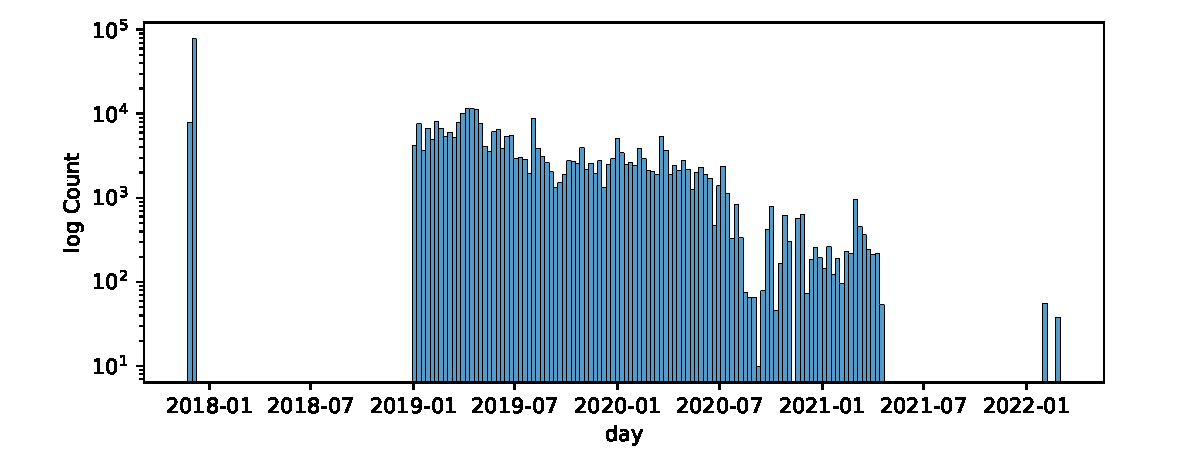
\includegraphics[width=\linewidth]{figure/saleauction count 1.pdf}
	\caption{saleAction函数调用频次}
	\label{fig:saleauction count 1}
\end{figure}

因此更换思路,从hive数据库中获取需要的数据。数据获取过程分为两个部分:
\begin{enumerate}
\item 从transactions数据库中获取地址为Core、SaleAuction的交易数据,并通过解析input来得到函数的输入。

\item 从logs数据库中获取地址为Core的log数据,通过解析data来获得log的输入。
\end{enumerate}


由于按照日期等于“\%Y-\%m-\%d”检索速度较快,且如果一次性检索过多日期会触发100,000的数据量上限,因此采取网络自动化的方法,按日期检索。其SQL语句如listing~\ref{SQL:2}所示。%网络自动化代码如\ref{section:selenium code}节所示。
最后将分日期获取的1865个csv文件合并为一个文件,就获得了合约地址下的所有交易。最终生成了三个csv文件,分别为Core.csv,SaleAuction.csv和log.csv。


\begin{lstlisting}[language=Sql,caption=获取智能合约地址下的所有数据,label=SQL:2]
SELECT
  * 
FROM 
  nifi_ethereum.transactions 
WHERE 
  to_address = "0x06012c8cf97bead5deae237070f9587f8e7a266d"
  AND day ="%Y-%m-%d"
 \end{lstlisting}

\section{研究主题}

\subsection{CryptoKitties的市场活跃度}
市场活跃度,即市场中产品交易的数量和频率,是衡量市场或产品需求和流通状况的重要指标。市场活跃度高意味着需求和积极性高,说明市场或产品受欢迎,价值和发展潜力较高。

图\ref{fig:saleauction count}-图\ref{fig:givebrith count}展示了2017年11月至2023年1月的市场活跃度相关数据。其中横轴表示时间,14天为一个单位;纵轴表示函数调用频次,以对数坐标呈现。

图\ref{fig:saleauction count}和图\ref{fig:bid count}展示了销售拍卖的相关数据。可以看到,从2017年至2023年,市场上的交易数量总体上呈现下降趋势,2018年一整年,拍卖数量和成交数量都在每14天1万左右;而到了2022年下半年,拍卖数量和成交数量下降至每14天120-150。

\begin{figure}[!htbp]
	\centering
	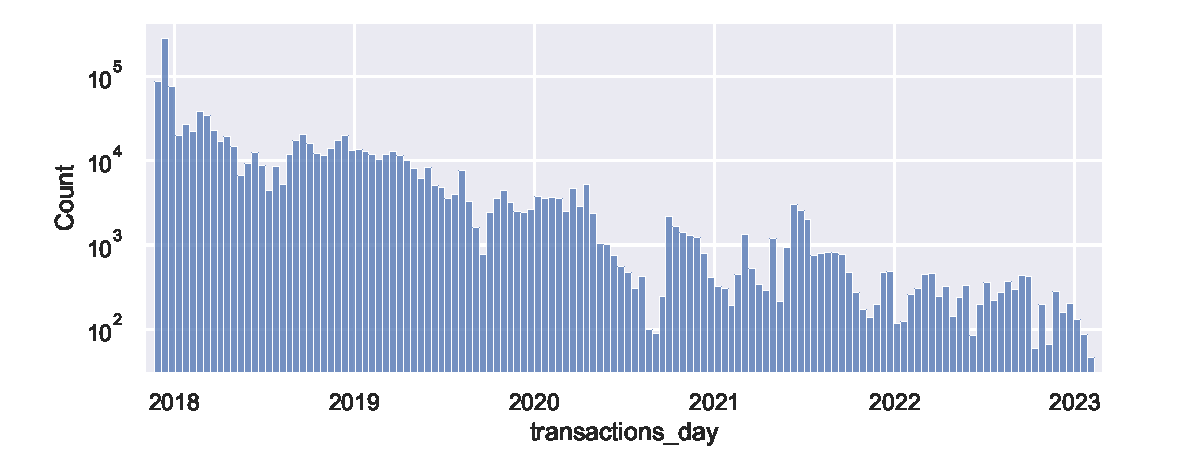
\includegraphics[width=\linewidth]{figure/saleauction count.pdf}
	\caption{创建销售拍卖的频次}
	\label{fig:saleauction count}
\end{figure}
\begin{figure}[!htbp]
	\centering
	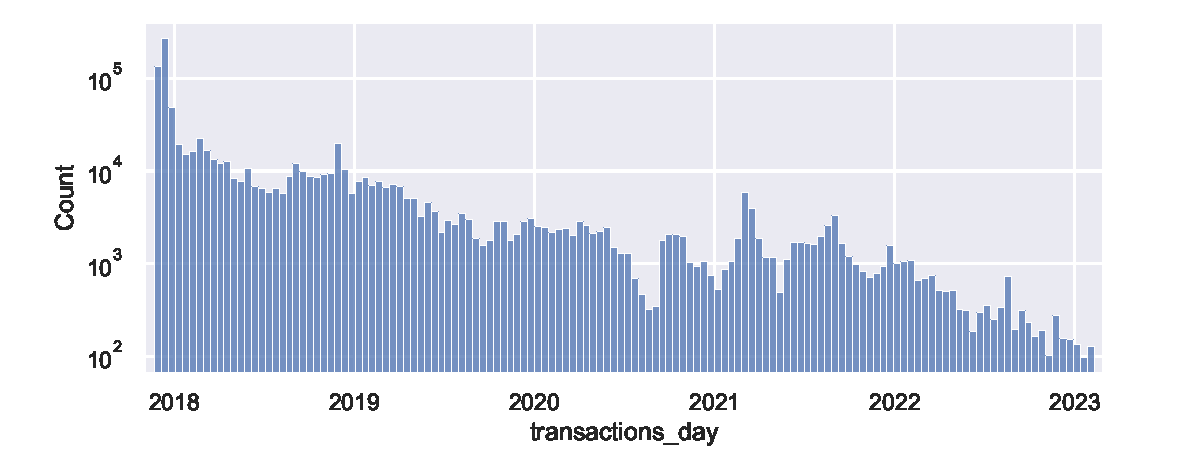
\includegraphics[width=\linewidth]{figure/bid count.pdf}
	\caption{销售拍卖成功数量}
	\label{fig:bid count}
\end{figure}

图\ref{fig:siringauction count}和图\ref{fig:bidOnSA count}展示了生育拍卖的相关数据。可以看到,从2017年至2022年,拍卖数量和成交数量在整体上呈现下降趋势,逐步从2018年的每14天1600次下降至2022年的每14天10次。在2022年以后,几乎不再有人购买猫的交配权。但是拍卖次数在短暂的归零以后,又恢复到了每14天10次的水平。
\begin{figure}[!htbp]
	\centering
	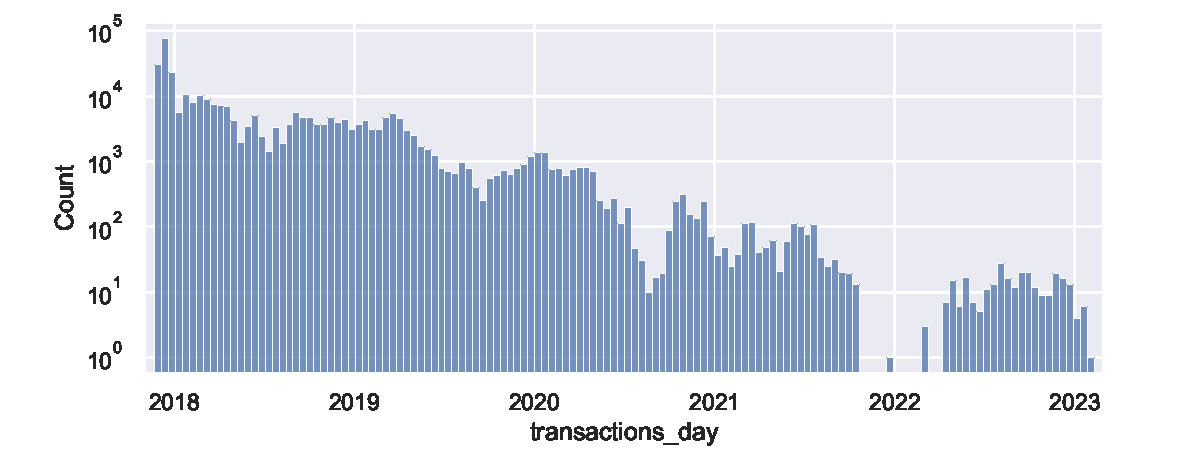
\includegraphics[width=\linewidth]{figure/siringauction count.pdf}
	\caption{创建生育拍卖的频次}
	\label{fig:siringauction count}
\end{figure}
\begin{figure}[!htbp]
	\centering
	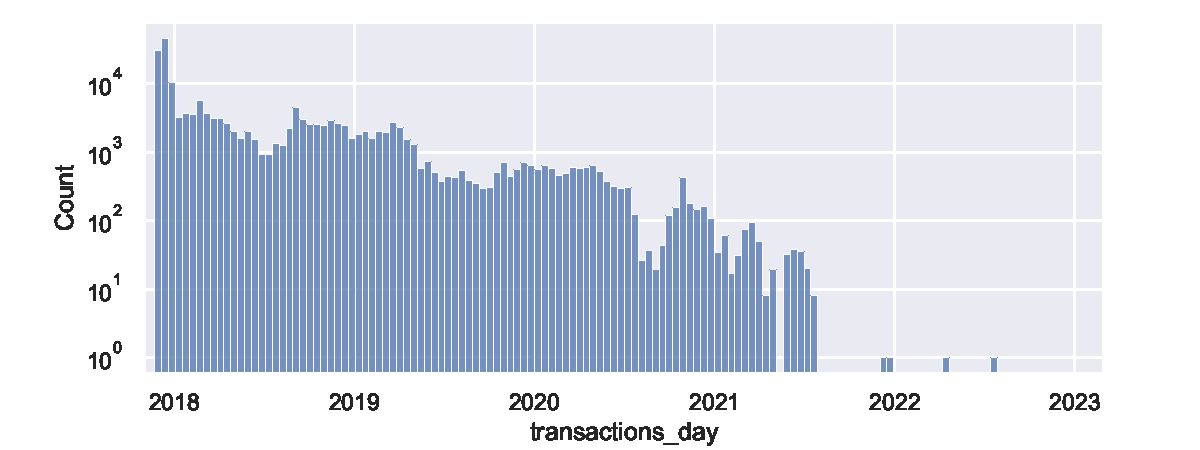
\includegraphics[width=\linewidth]{figure/bidOnSA count.pdf}
	\caption{生育拍卖成功数量}
	\label{fig:bidOnSA count}
\end{figure}

图\ref{fig:givebrith count}展示了出生小猫的数量。在2017年-2018年,出生数量的波动量较大,从每14天10万只到每14天10只不等;2019年至2020年,每14天的出生数量维持在1万只左右;但是到了2022年,每14天的出生数量下降至100只左右。

\begin{figure}[!htbp]
	\centering
	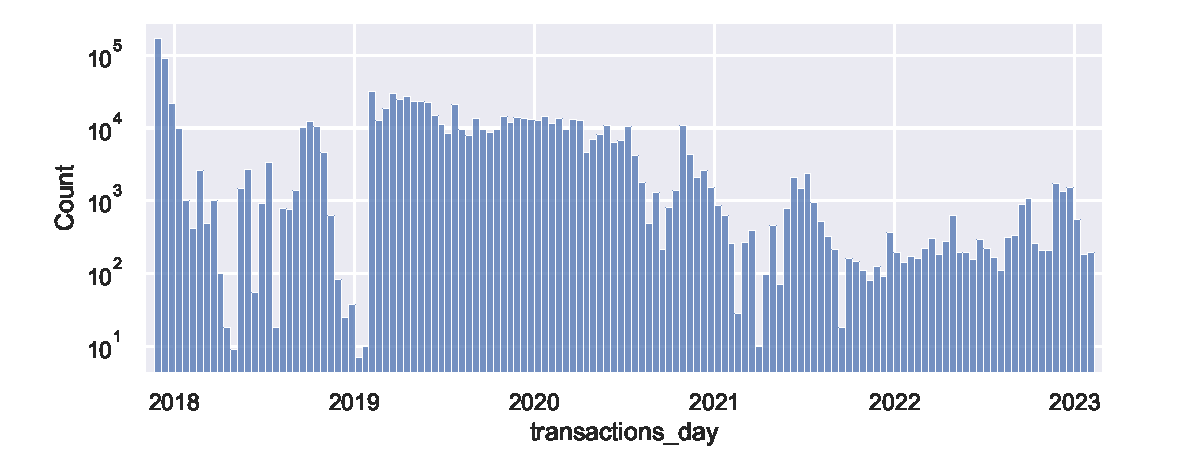
\includegraphics[width=\linewidth]{figure/givebrith count.pdf}
	\caption{出生小猫数量}
	\label{fig:givebrith count}
\end{figure}

总的来说,CryptoKitties从2017年11月23号首发,在同年12月即达到巅峰,并在2018年一整年维持在了一个较高的水平,但是由于其玩法单一,以投机为主,在经历了短暂的高热度后市场活跃度开始逐渐走低,交易量显著减少。

\subsection{CryptoKitties的市场价格波动}
市场价格波动是指市场价格在一段时间内不断变动的情况。市场价格波动代表了市场供求关系的变化。当市场需求量增加,市场价格会上涨;当市场供给量增加,市场价格则会下降。市场价格波动还反映了市场对于公司、产品、行业的信心度。当市场对公司、产品、行业充满信心,市场价格会上涨;当市场对公司、产品、行业信心不足,市场价格则会下降。

图\ref{fig:price ETHsP}-图\ref{fig:price USDP}展示了从2017年11月至2023年1月的市场价格波动的相关数据,其中横轴表示时间,以天为单位;纵轴表示价格,以对数坐标呈现。其中实线表示价格的平均值,半透明的区域表示当天的价格区间。

图\ref{fig:price ETHsP}和图\ref{fig:price USDsP}分别展示了以以太币和以美元结算的拍卖开始价格,其中拍卖开始价格大于100亿美元的作为异常值被删掉,没有显示在图中。其中以美元为结算的价格波动图中展示出了较为明显的规律。总体上呈现出先下降、后上升、再下降的趋势。拍卖开始价格在一定程度上表明了用户对于市场的信心,一个较高的拍卖开始价格表明用户更有信心卖出高价。在2021年下半年后,拍卖开始价格呈现明显的下降趋势,表明用户对于市场的信心正在逐渐下降,这和市场活跃度的降低相吻合。


\begin{figure}[!htbp]
	\centering
	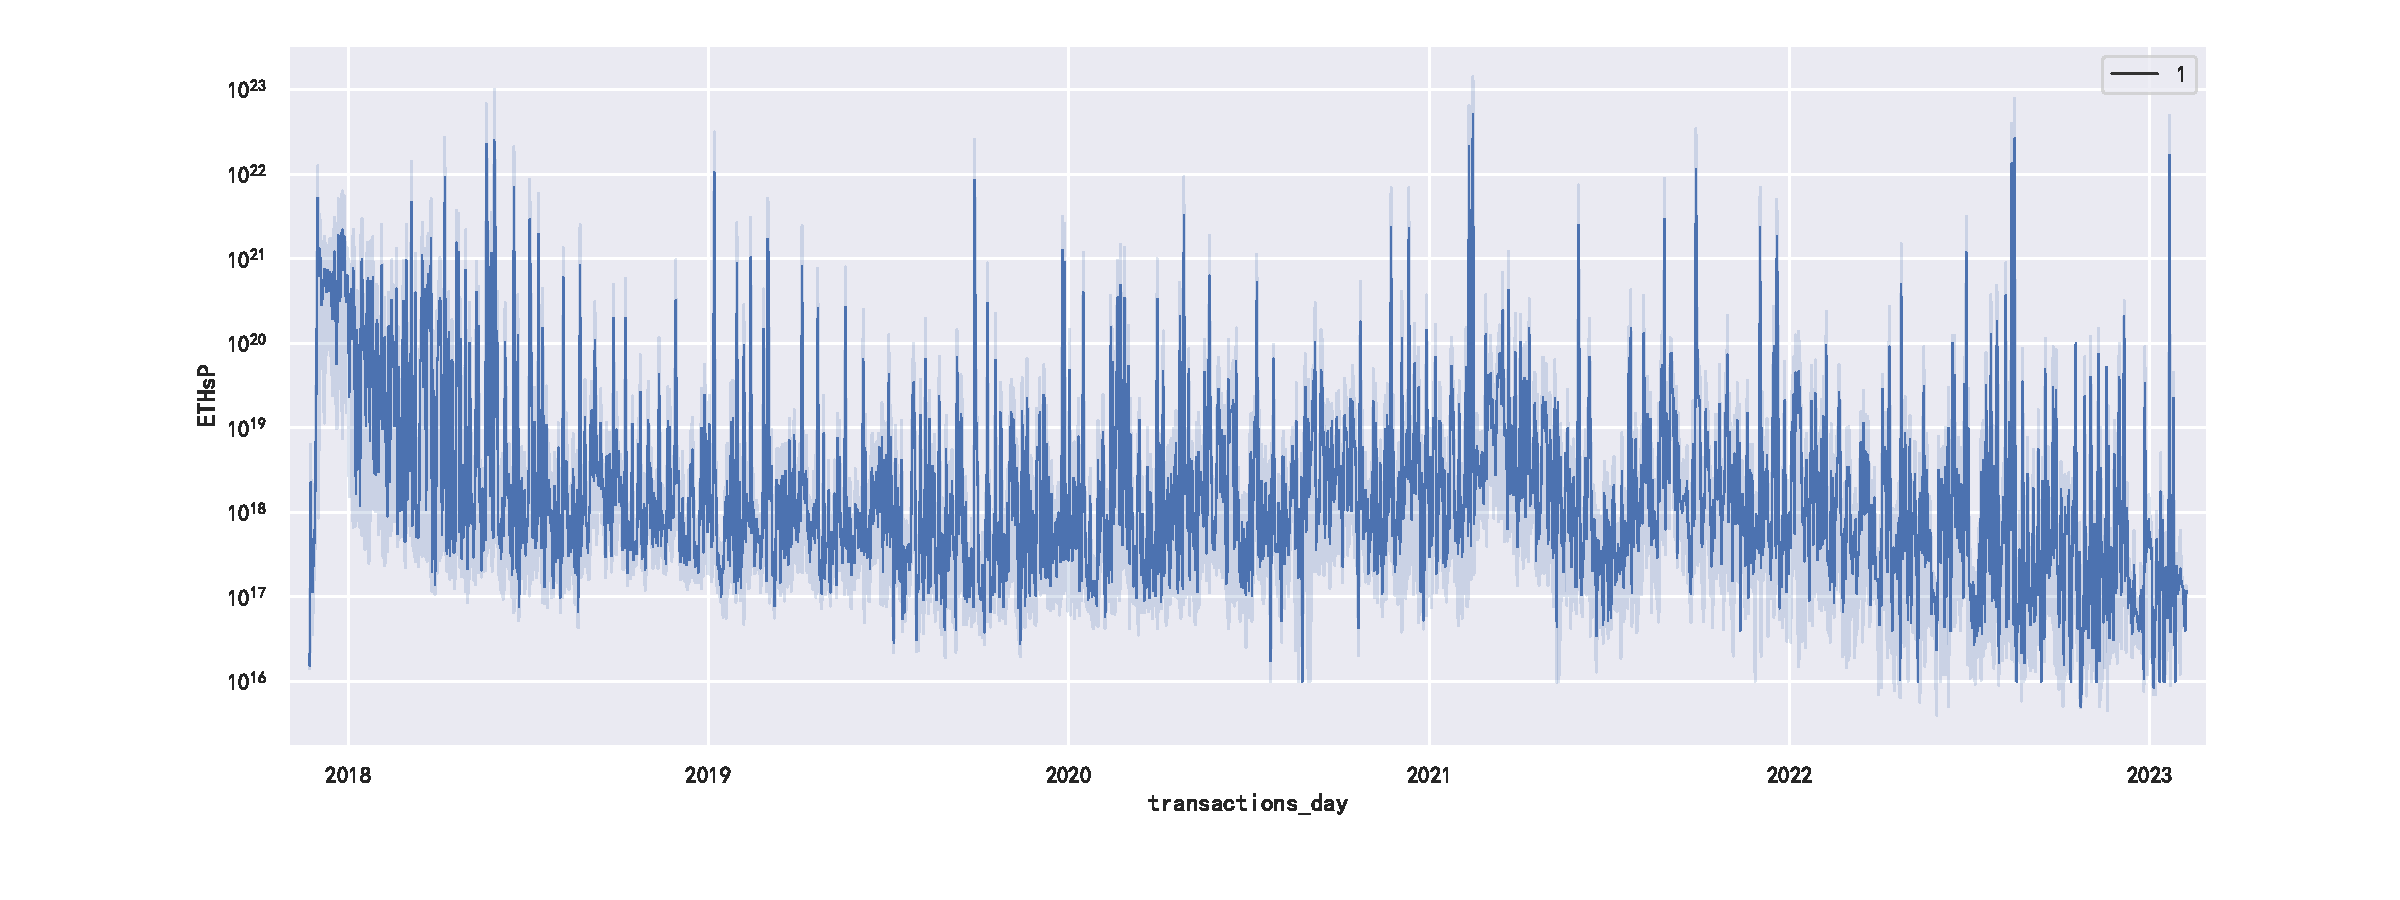
\includegraphics[width=\linewidth]{figure/price ETHsP.pdf}
	\caption{拍卖开始价格(Wei)}
	\label{fig:price ETHsP}
\end{figure}
\begin{figure}[!htbp]
	\centering
	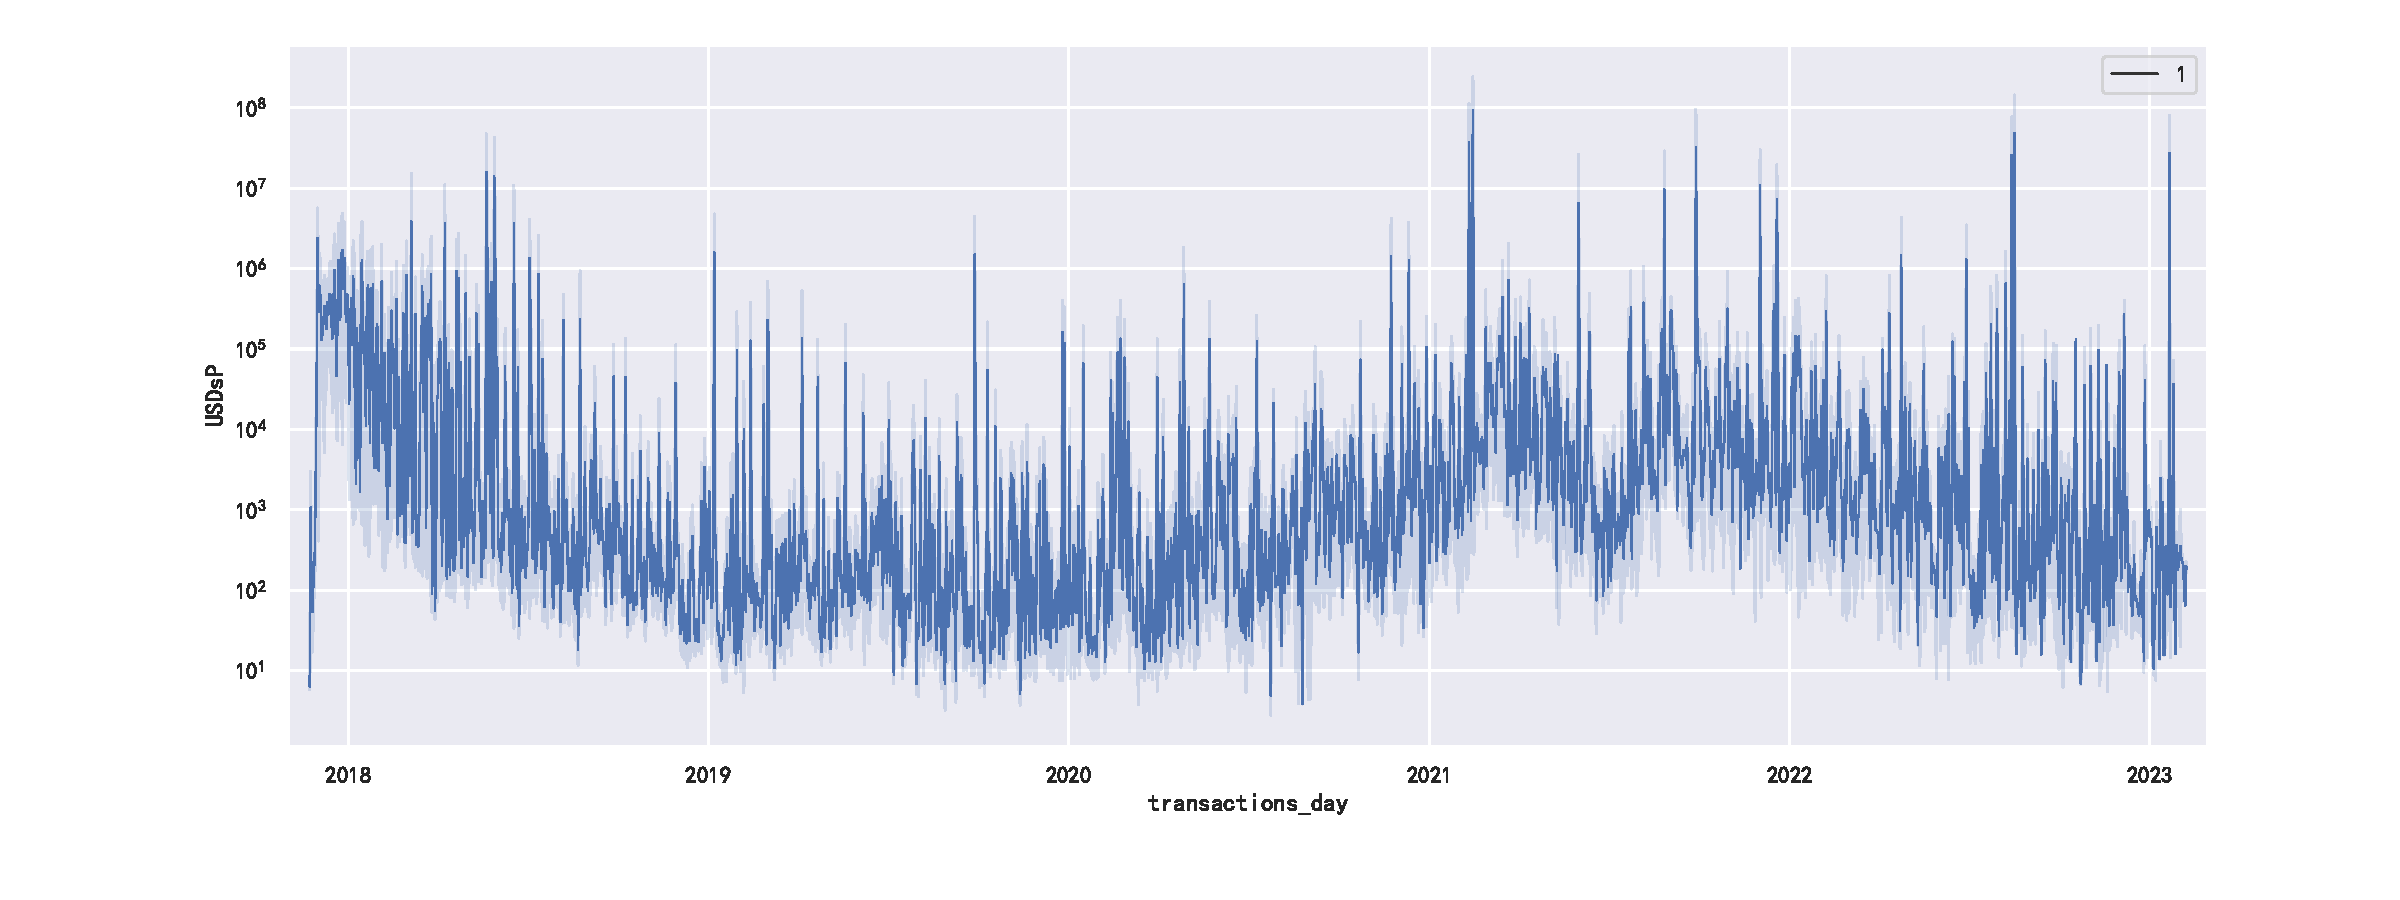
\includegraphics[width=\linewidth]{figure/price USDsP.pdf}
	\caption{拍卖开始价格(USD)}
	\label{fig:price USDsP}
\end{figure}


图\ref{fig:price ETHeP}和图\ref{fig:price USDeP}分别展示了以以太币和以美元结算的拍卖结束价格。其中拍卖结束价格大于100亿美元的作为异常值被删掉,没有显示在图中。拍卖结束价格有三种选择:比开始价格低,等于开始价格和比开始价格高,不同选择的比例如图\ref{fig:bid pie}所示。虽然CryptoKitties没有限制开始拍卖价格一定要比结束拍卖价格高,但由于其拍卖模式,有82.6\%的人选择了荷兰式拍卖(即降价式拍卖),有12.5\%的人选择了定价拍卖,仅有4.8\%的人选择了增价拍卖。因此拍卖的结束价格在一定程度上表明了拍卖者对于拍卖的猫的价值判断,而高出结束价格的部分代表某种消费者剩余。如果拍卖价格低于拍卖者的心理预期价值,拍卖者宁可流拍。

和拍卖开始价格类似,拍卖结束价格在以美元结算的情况下体现出了较强的规律性,拍卖结束价格先下降、后上升、再下降。表明2022年以来,CryptoKittie上的猫的价值正在逐渐下降。

但值得注意的是,虽然目前呈现下降趋势,其平均价格仍然比2019年的时候高。这主要是受到了供需关系的影响:图\ref{fig:createMinusBid}展示了每日创建拍卖数量与竞拍成功数量之差,由于拍卖往往持续数天,所以取值有可能为负数。图中只展示了-500-500的区间。可以看到一开始由于有大量的猫在市场上流通,所以分布较为分散且远离0,而到2022年以后,每日创建拍卖数量与竞拍成功数量之差在0附近波动,这表明需求大于供应,几乎所有的供应都被消化掉了。这种供给短缺造成了价格仍在高位。

\begin{figure}[!htbp]
	\centering
	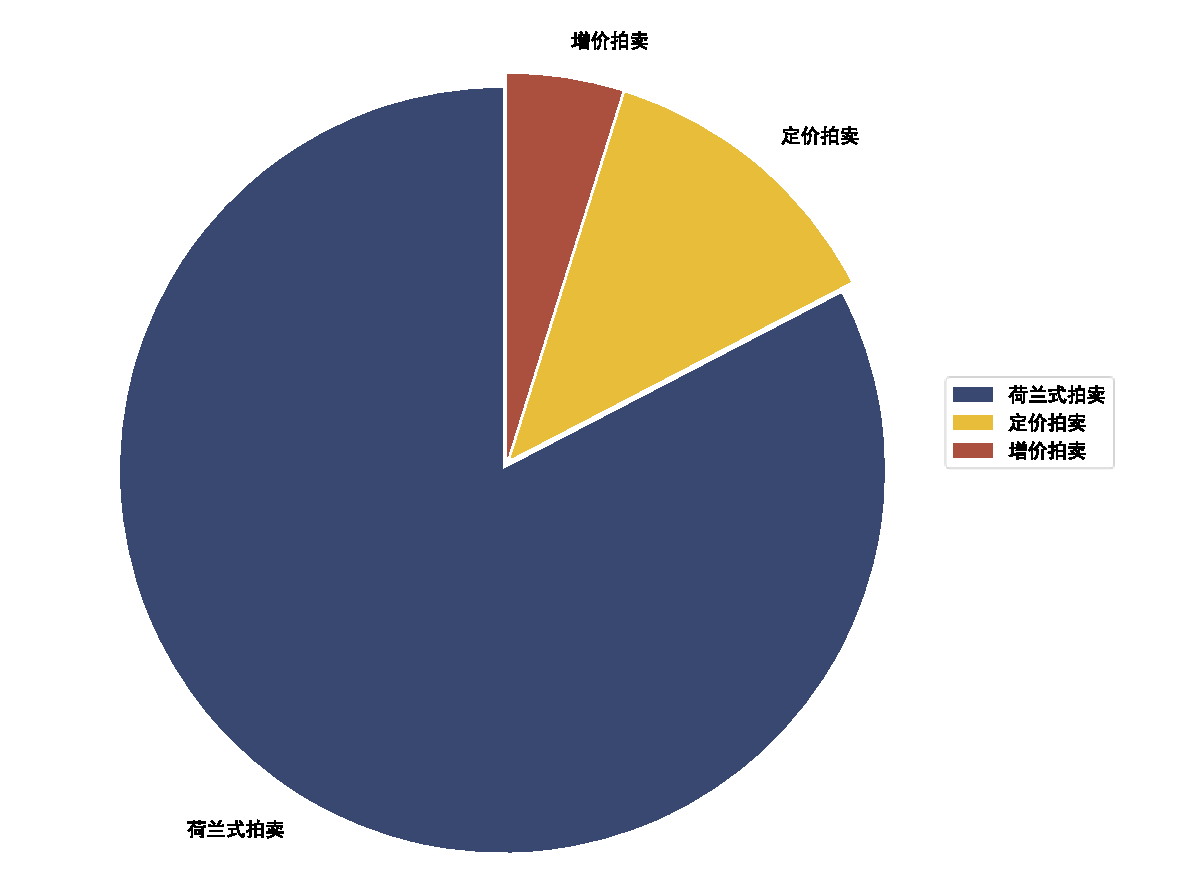
\includegraphics[width=3in]{figure/bid pie.pdf}
	\caption{不同拍卖的比例}
	\label{fig:bid pie}
\end{figure}

\begin{figure}[!htbp]
	\centering
	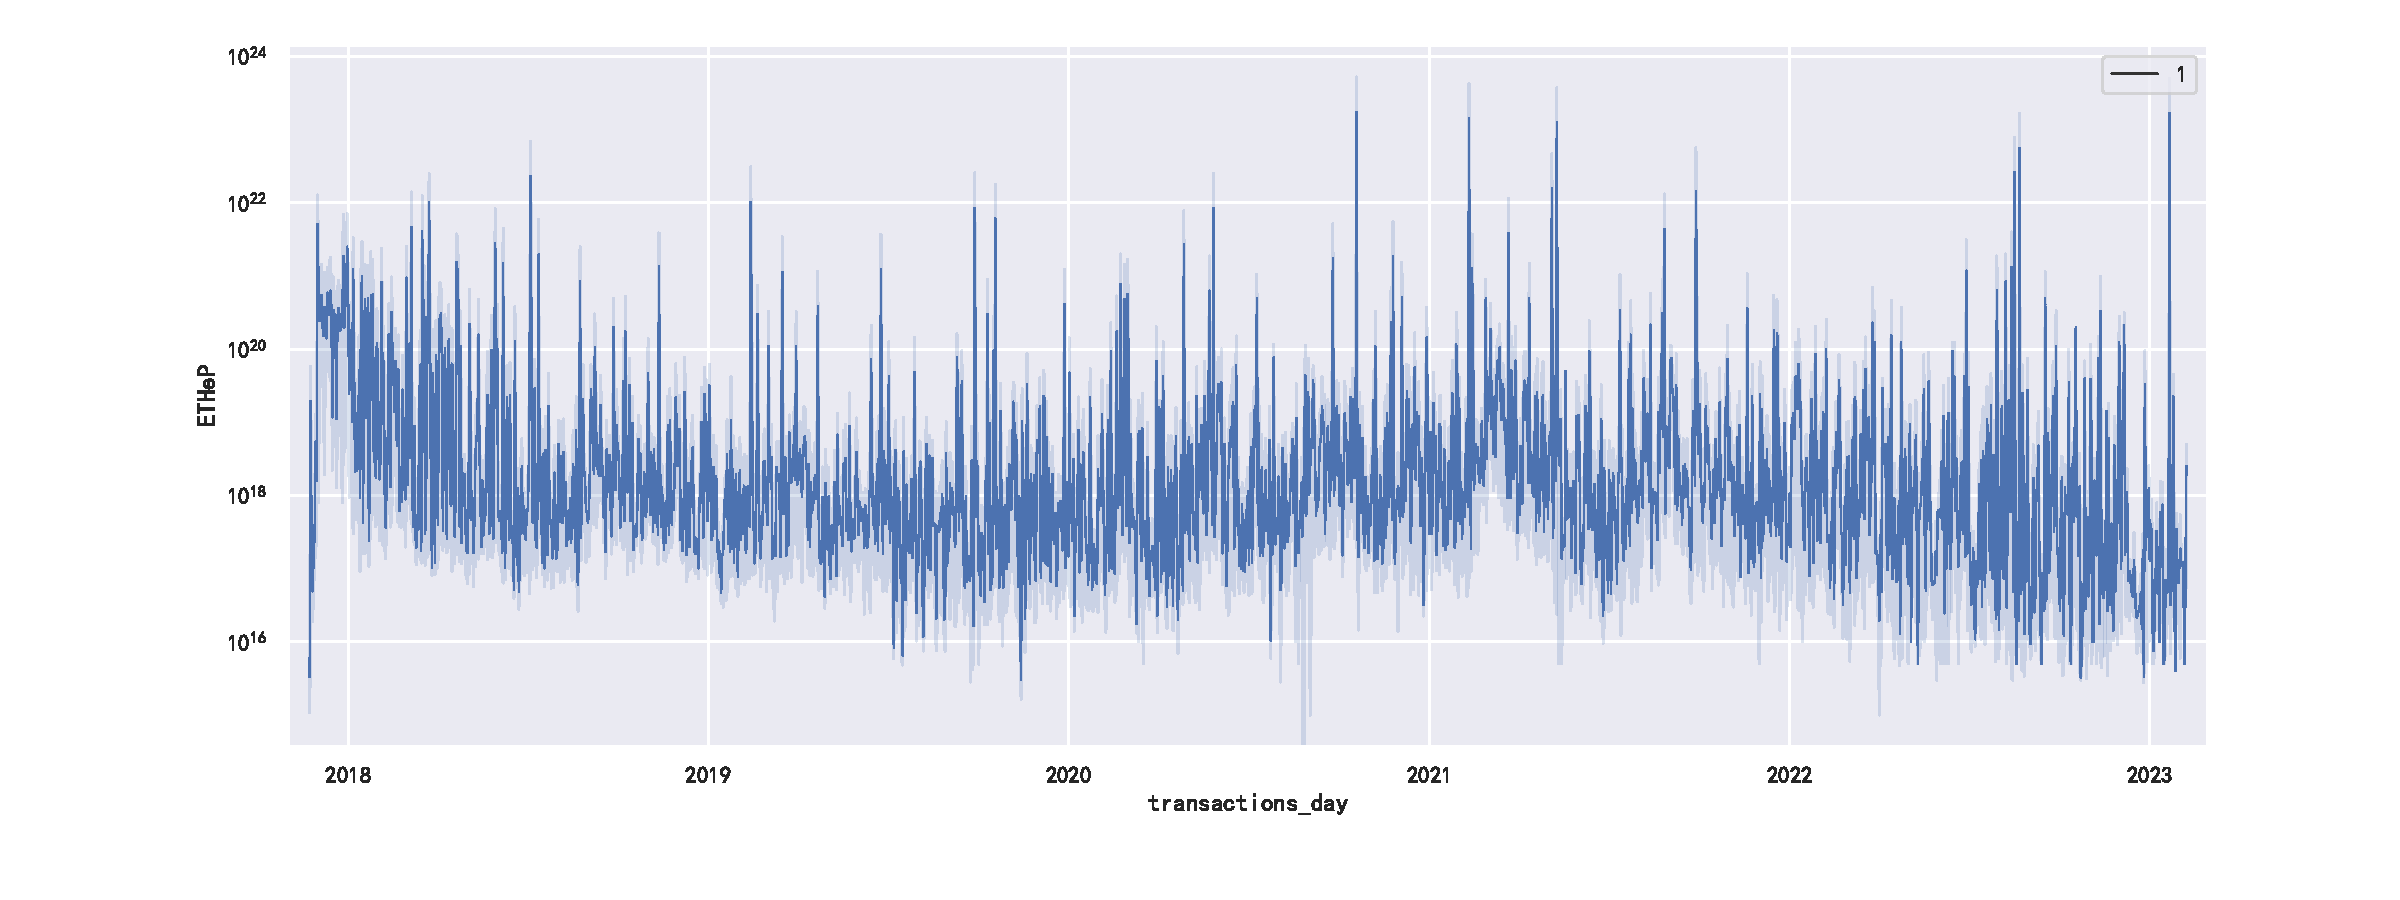
\includegraphics[width=\linewidth]{figure/price ETHeP.pdf}
	\caption{拍卖结束价格(Wei)}
	\label{fig:price ETHeP}
\end{figure}
\begin{figure}[!htbp]
	\centering
	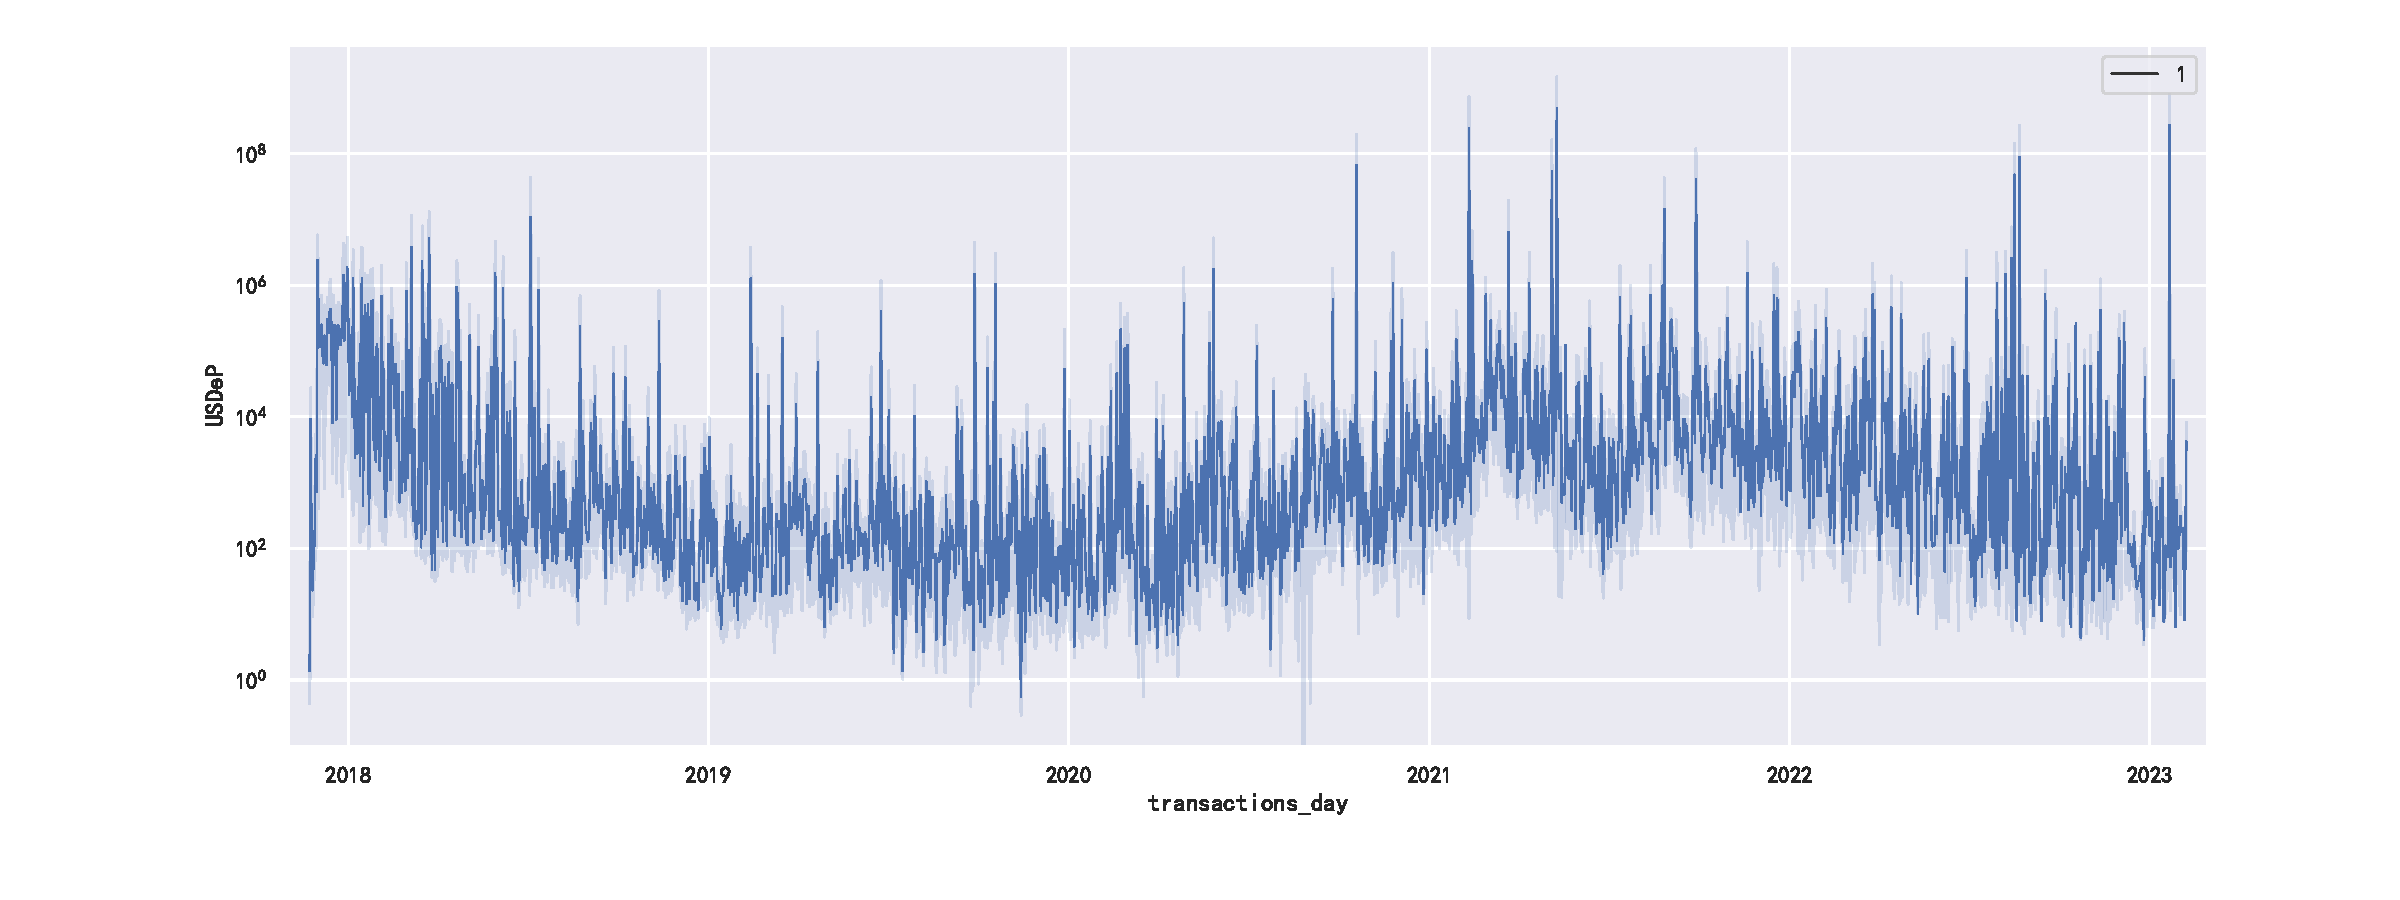
\includegraphics[width=\linewidth]{figure/price USDeP.pdf}
	\caption{拍卖结束价格(USD)}
	\label{fig:price USDeP}
\end{figure}

\begin{figure}[!htbp]
	\centering
	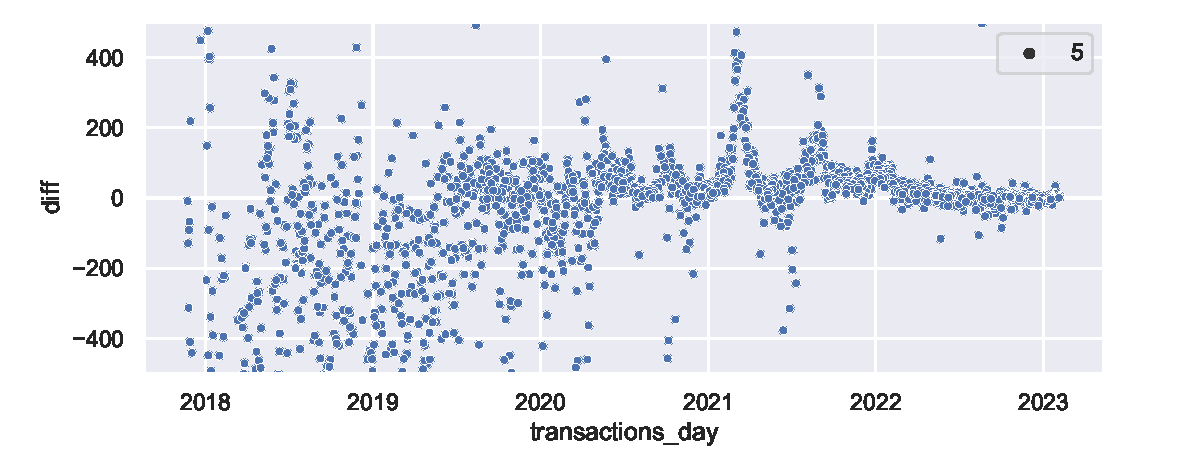
\includegraphics[width=\linewidth]{figure/createMinusBid.pdf}
	\caption{每日创建拍卖数量与竞拍成功数量之差}
	\label{fig:createMinusBid}
\end{figure}



图\ref{fig:price ETHP}和图\ref{fig:price USDP}分别展示了以以太币和美元结算的拍卖成交价格。可以看到,2018年成交价格在15美元左右,2019年跌至4美元左右,从2020开始到2021年下半年,随着以太币(ETH)价格的突飞猛涨,成交价格也提升到了一百美元左右。2021年下半年以后,成交价格逐渐回落到18年的水平。



\begin{figure}[!htbp]
	\centering
	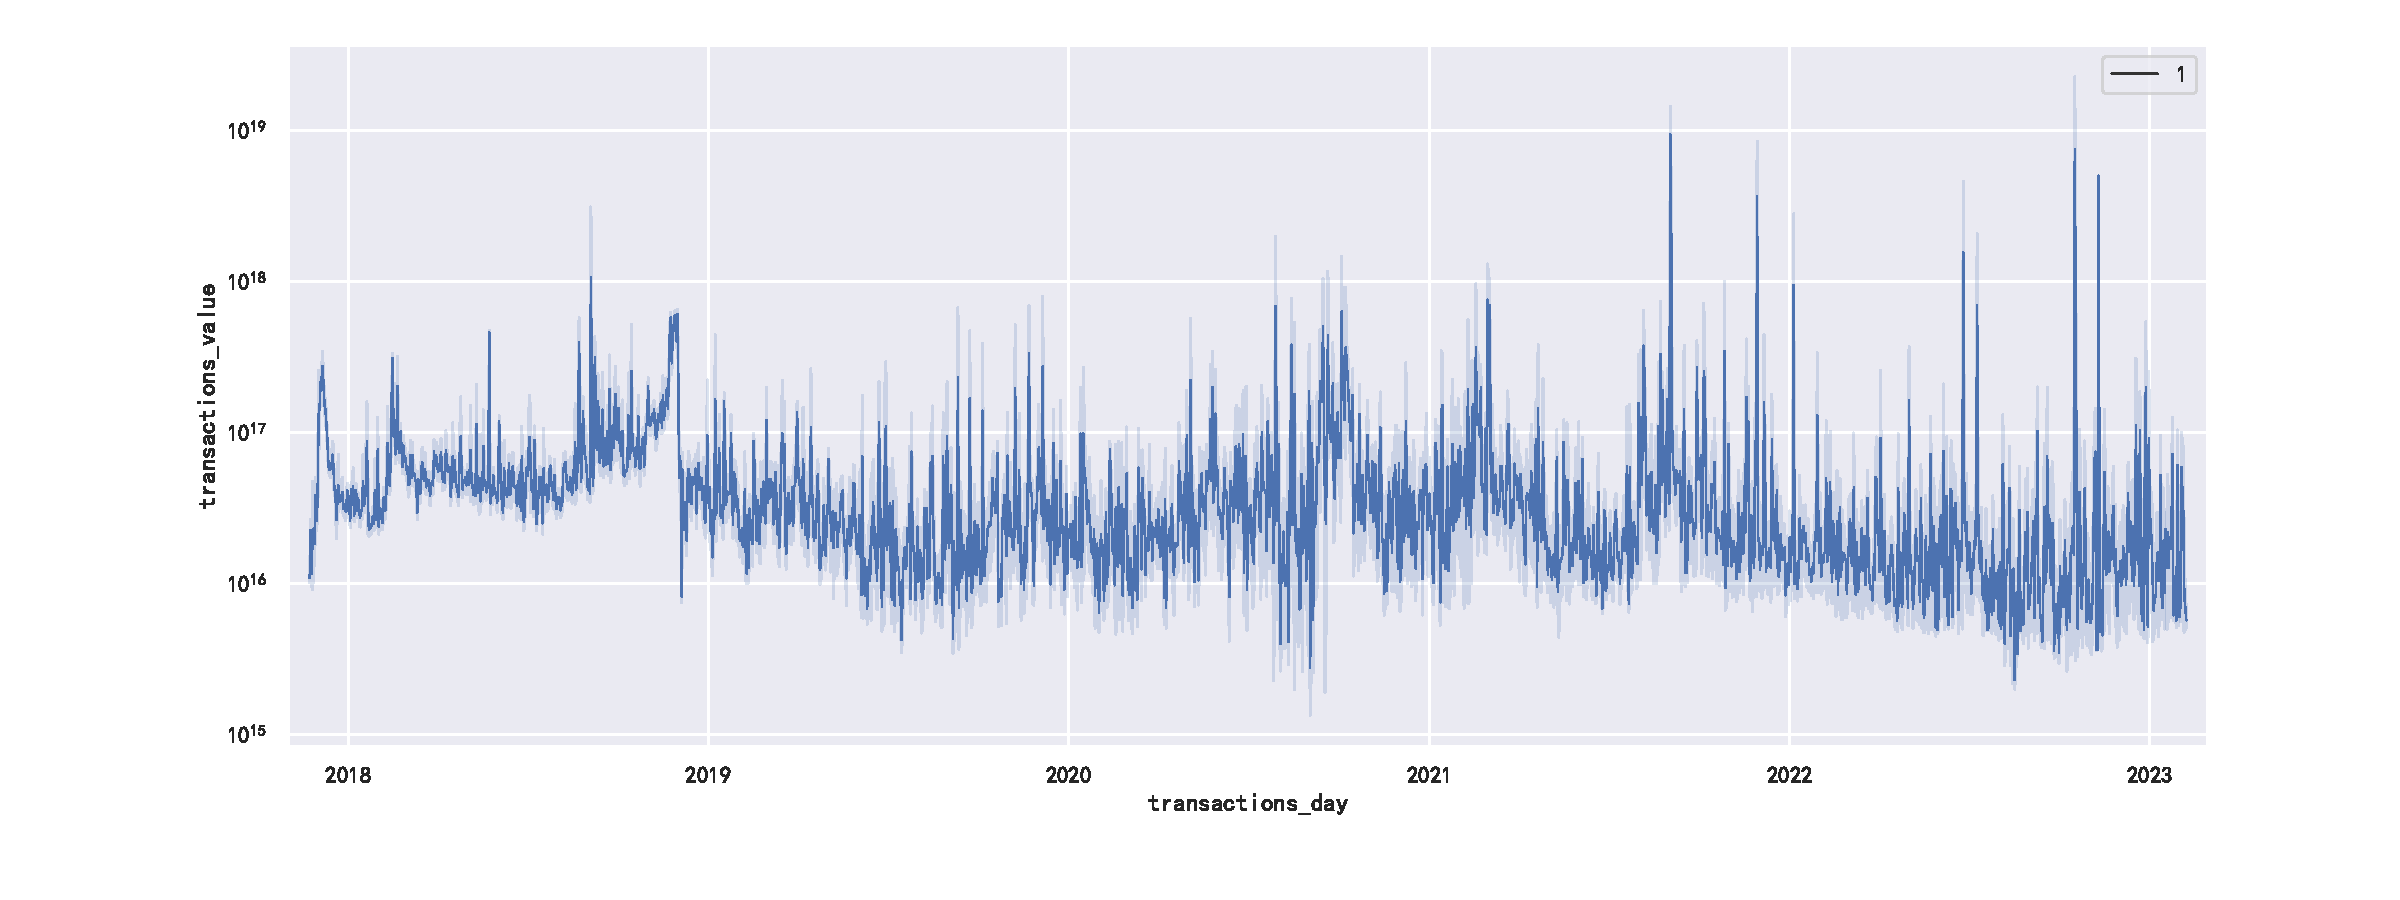
\includegraphics[width=\linewidth]{figure/price transactions_value.pdf}
	\caption{成交价格(Wei)}
	\label{fig:price ETHP}
\end{figure}
\begin{figure}[!htbp]
	\centering
	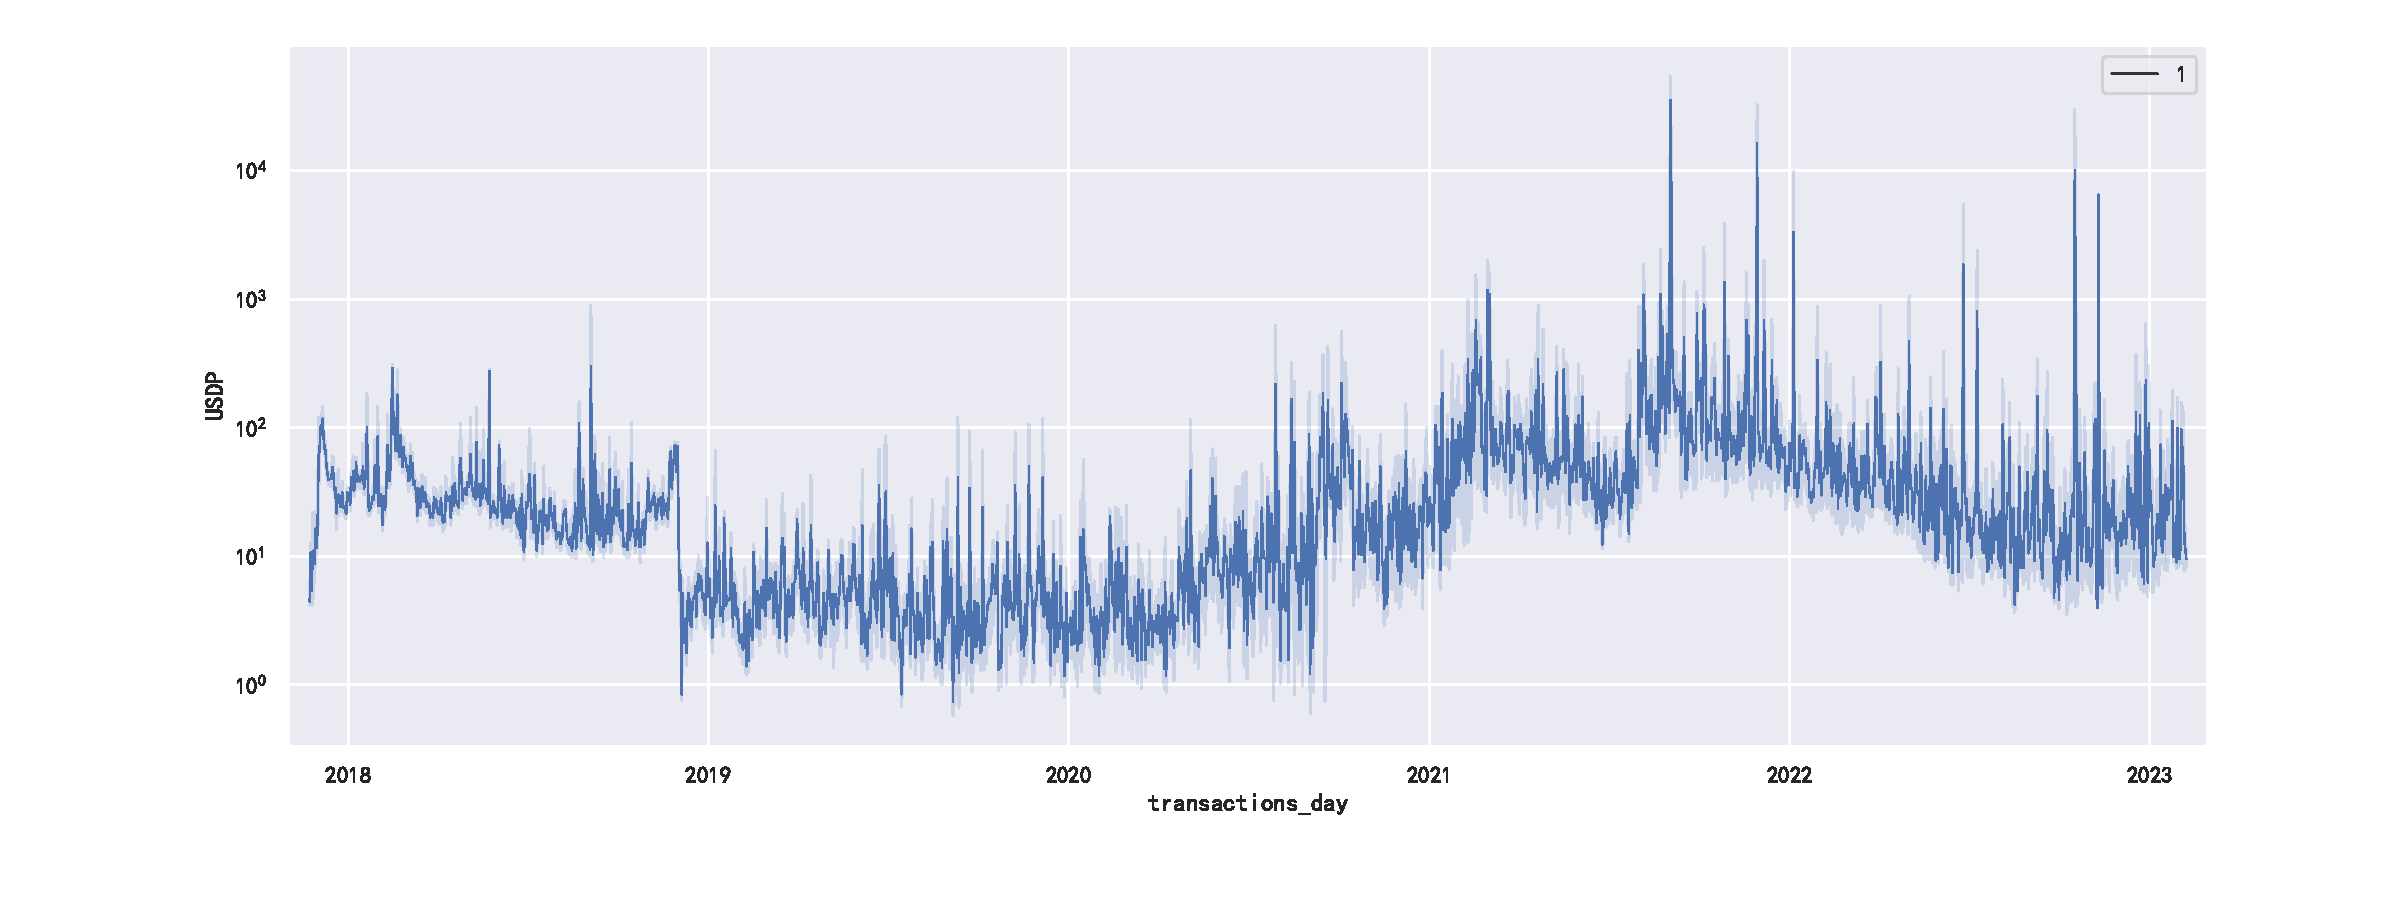
\includegraphics[width=\linewidth]{figure/price USDP.pdf}
	\caption{成交价格(USD)}
	\label{fig:price USDP}
\end{figure}


总的来说,CryptoKitties的拍卖价格受多方面影响。如用户对于市场的信心、市场活跃度、供需关系、以太币价格、猫的个体差异等等。受个体差异影响,成交价格波动较为剧烈,每日成交价的最高价和最低价可能相差20倍以上。但是从总体趋势而言,呈现先下降、后上升、再下降的趋势。并且虽然当前市场活跃度较低,价格也在走低,但是不论是拍卖开始价格、拍卖结束价格还是成交价格仍高于2019-2020年的价格。


\subsection{CryptoKitties的用户分析}
除了CryptoKitties的市场活跃度和市场价格变化外,用户交易频次的信息也十分重要。图\ref{fig:User Count hist}-图\ref{fig:User Count pie}展示了用户调用Core和SaleAuction两个合约中的函数的频次。由于调用函数在100以上的用户数量较少,所以仅展示了调用函数次数在100以内的数据。从图\ref{fig:User Count hist}中可以看到,有将近17,000名用户仅仅调用了一次,用户数量随着调用次数的增加而迅速减少。这表明大部分人将CryptoKitties当做一个非同质化代币(NFT)产品或者一款游戏,仅有小部分人以此牟利。图\ref{fig:User Count kde}展示了核密度估计的不同交易频次的用户数量的分布情况。

\begin{figure}[!htbp]
	\centering
	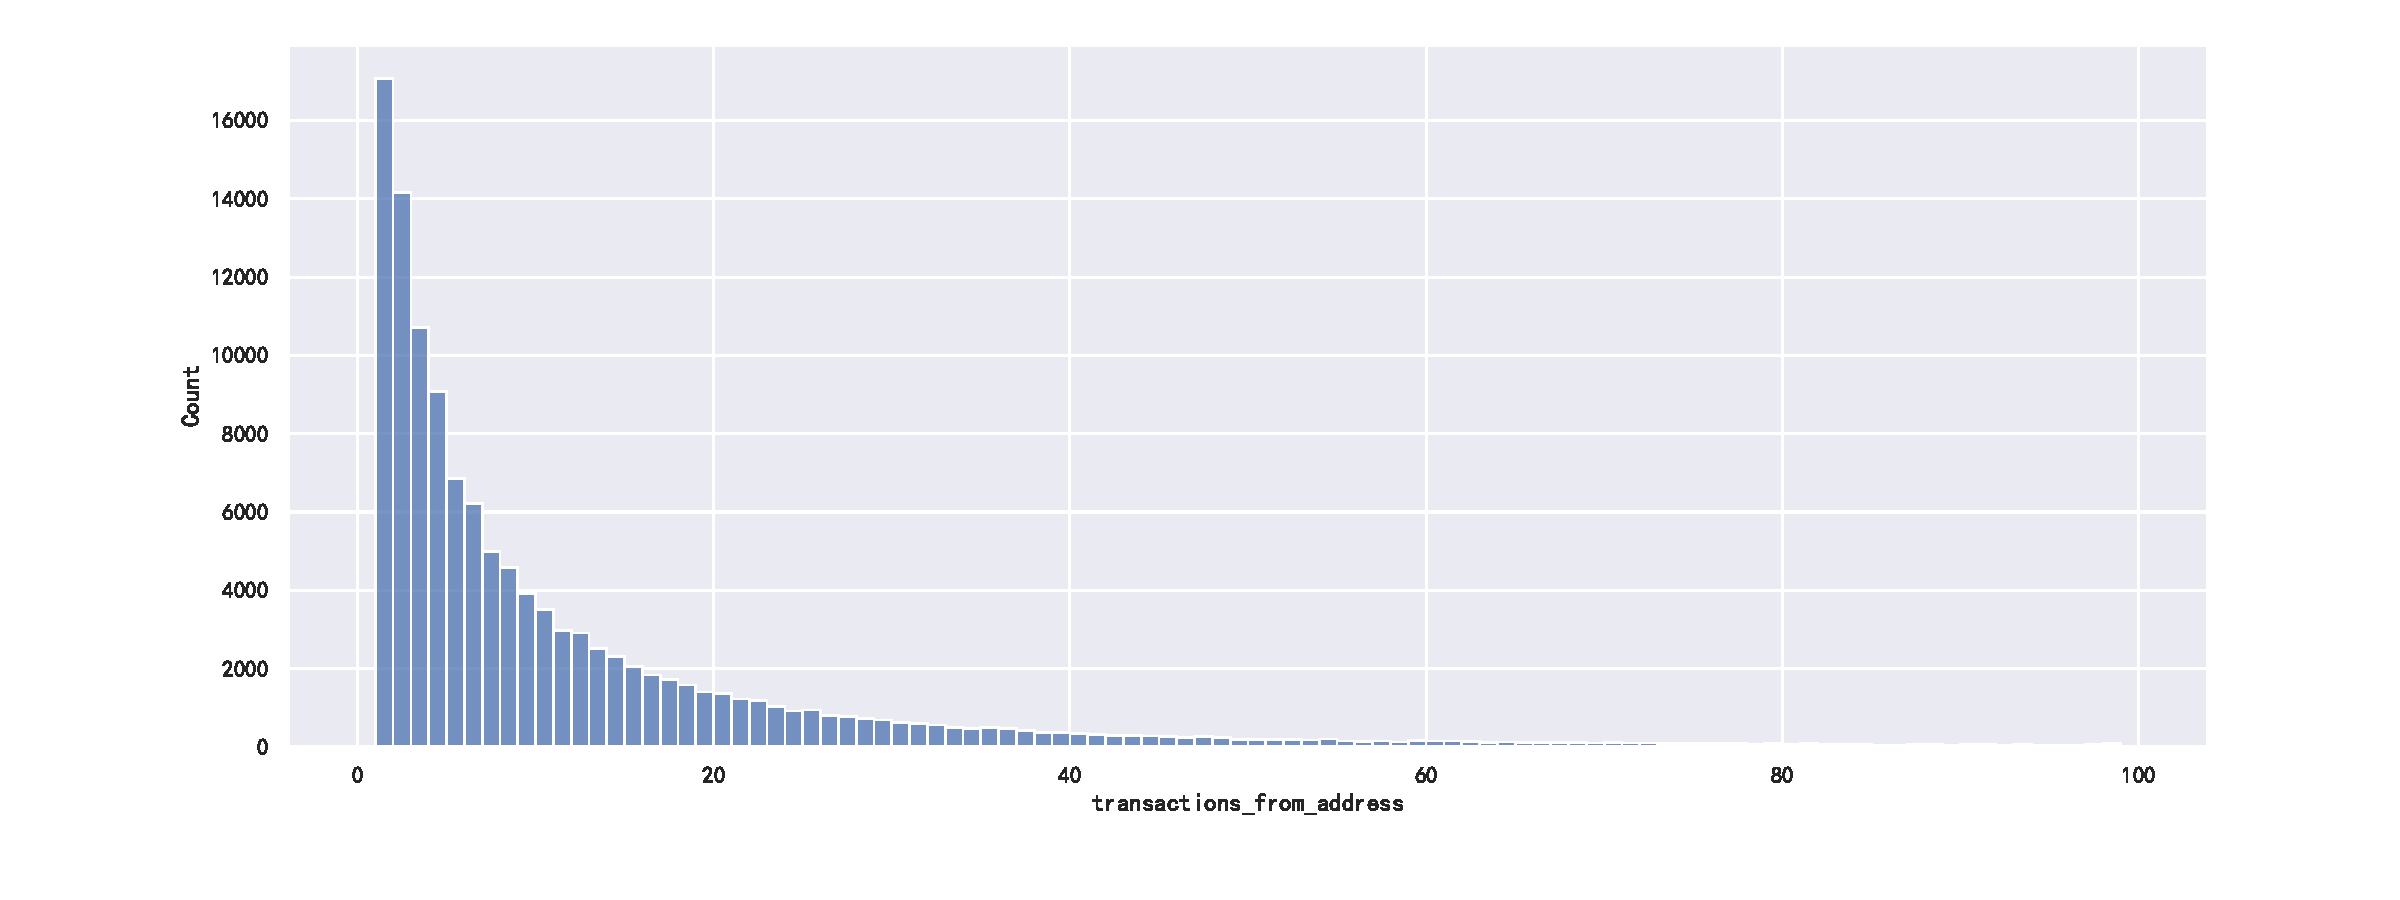
\includegraphics[width=\linewidth]{figure/User Count hist.pdf}
	\caption{用户调用函数的次数}
	\label{fig:User Count hist}
\end{figure}
\begin{figure}[!htbp]
	\centering
	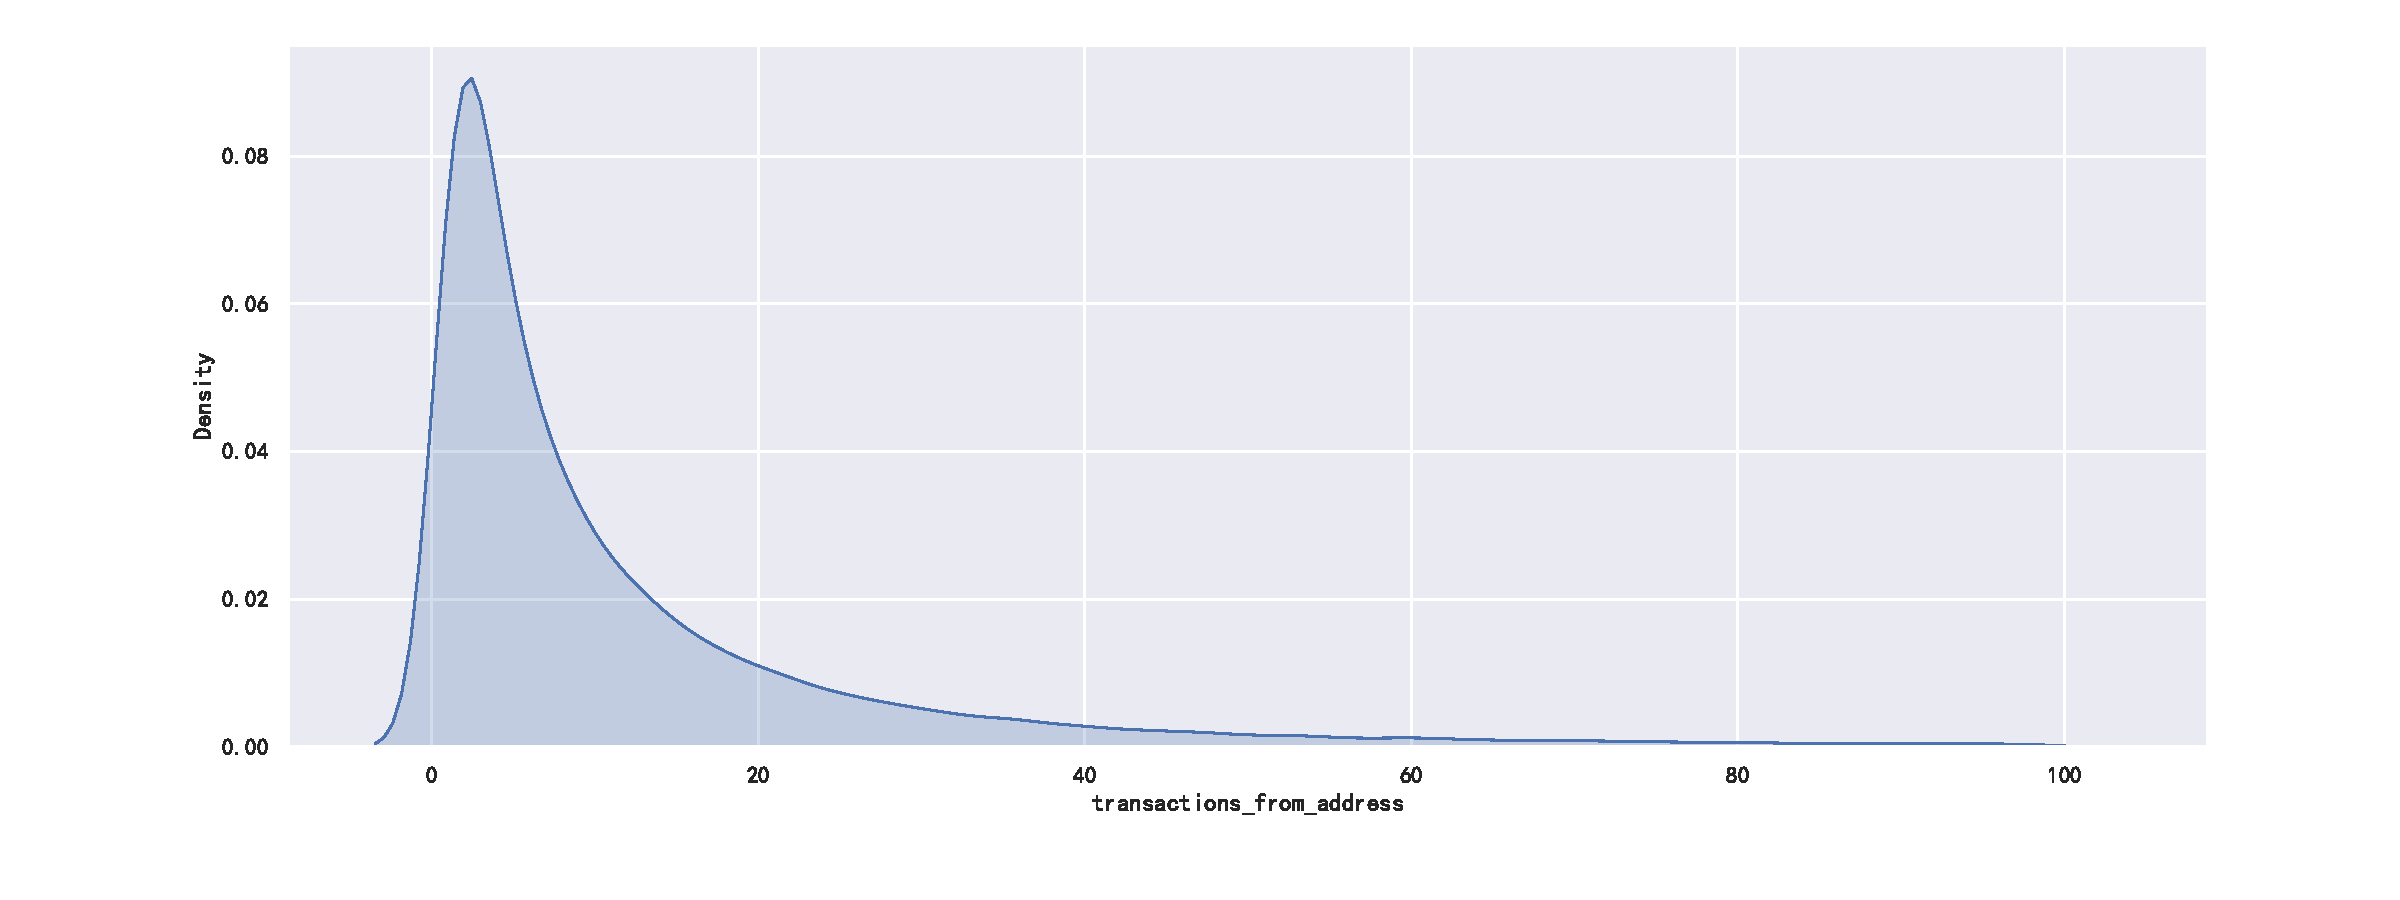
\includegraphics[width=\linewidth]{figure/User Count kde.pdf}
	\caption{用户调用函数的次数的核密度估计}
	\label{fig:User Count kde}
\end{figure}

图\ref{fig:User Count pie}展示了不同调用频次区间的用户数量所占比例。区间以指数划分(从$e^1$到$e^4$)。其中,1-3次占比32.9\%,4-8次占比24.9\%,9-20次占比22.1\%,21-55次占比13.3\%,55次以上占比6.8\%。

\begin{figure}[!htbp]
	\centering
	\includegraphics[width=3.5in]{figure/User Count pie.pdf}
	\caption{不同调用次数区间的比例}
	\label{fig:User Count pie}
\end{figure}

不同调用次数的用户群体中,其调用函数的占比也有所区别。图\ref{fig:user count function}显示了不同调用次数下,调用频次大于总调用数量5\%的函数的占比。可以看到,函数0x454a2ab3(bid)的调用比例随着调用次数的增加而逐渐减少,函数0xf7d8c883(breedWithAuto)的调用比例随着调用次数的增加而增加。0x3d7d3f5a(createSaleAuction)的调用比例随着调用次数的增加而增加,但是在大于55次的部分有所减少。0xed60ade6(bidOnSiringAuction)在9-55次的部分占比较多,其原因在于良好的种猫往往在重度玩家手中,且价格昂贵,轻度玩家如果想获得较好的基因则需要购买生育权。最后,0x88c2a0bf(Birth)的调用次数仅在调用频次大于55的群体中占比高于5\%,且以18.8\%的占比成为调用频次第二高的函数。


\begin{figure}[!h]
	\centering
	\subfigure[1-3]{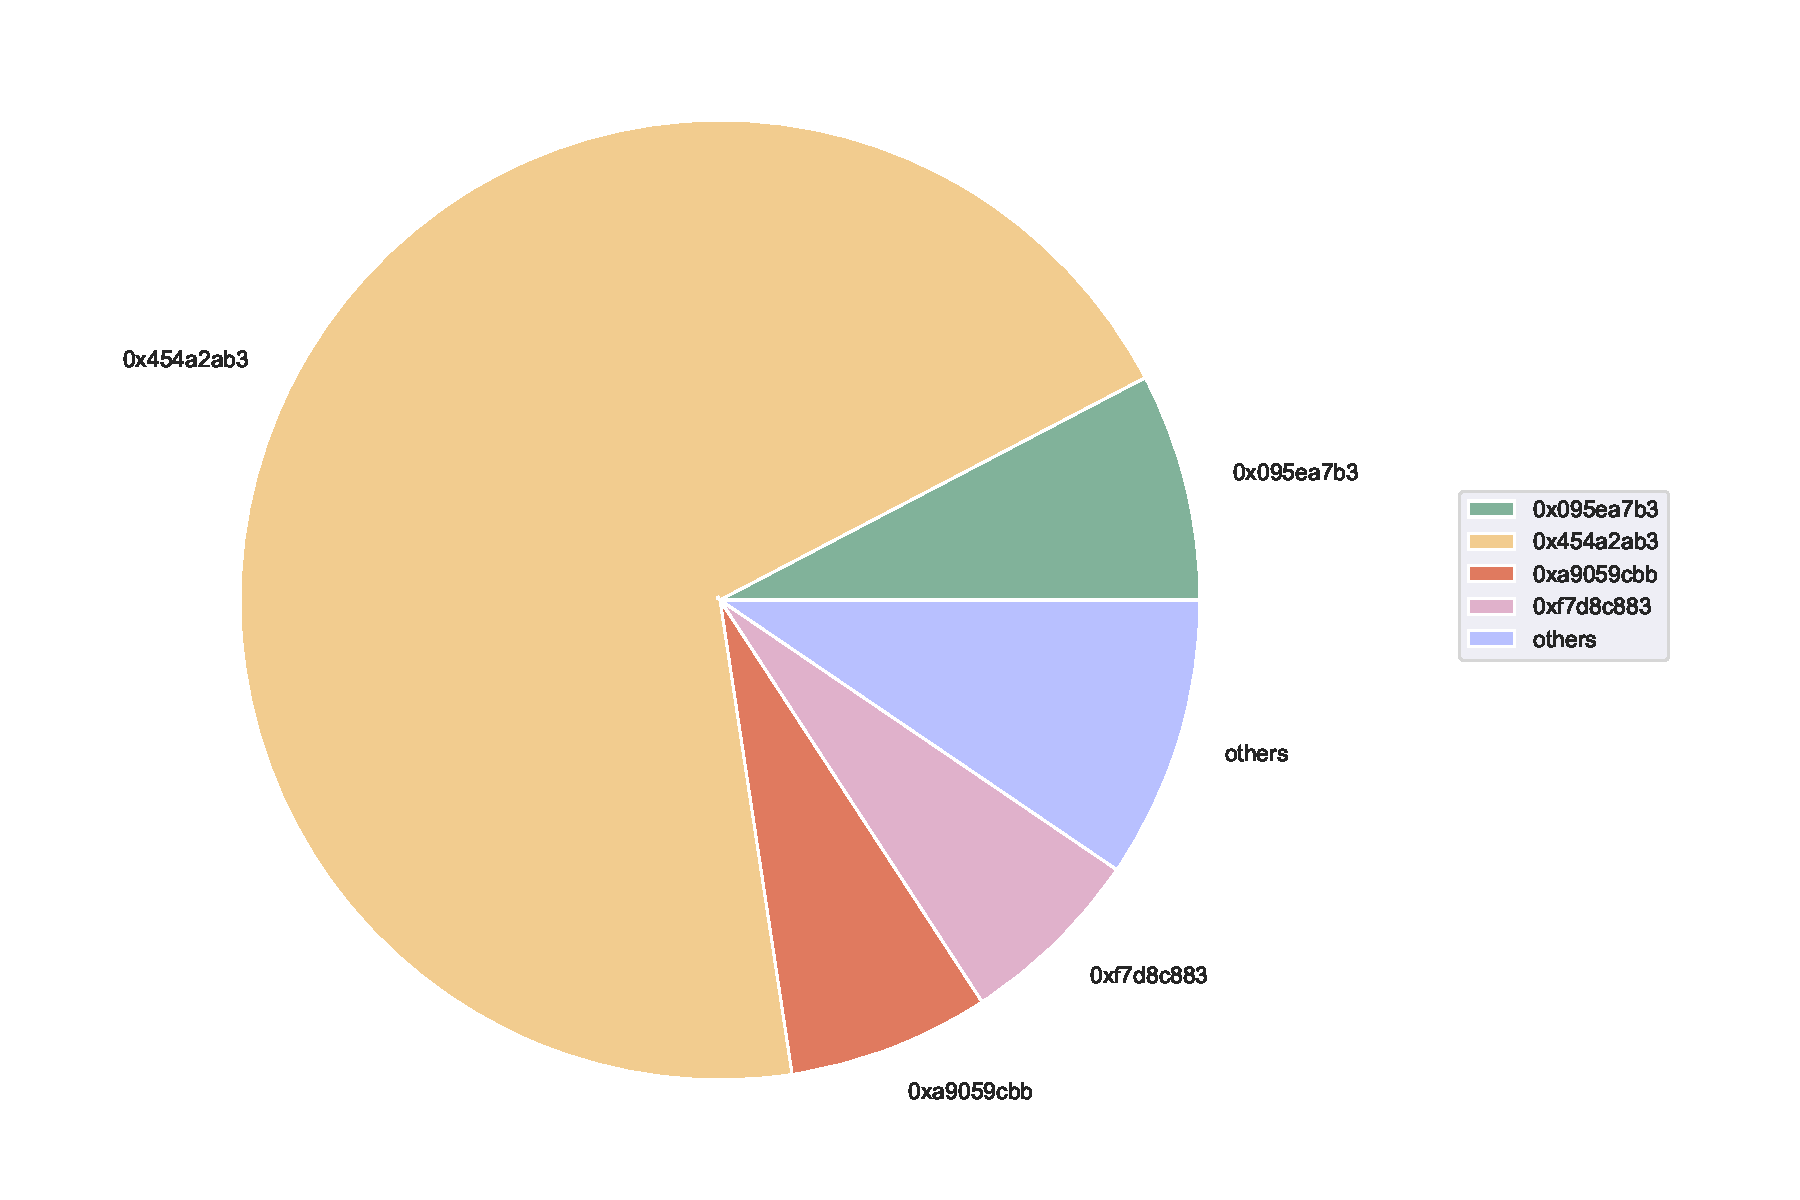
\includegraphics[height=2in]{figure/user count function0.pdf}}
	\hspace{0 pt}
	\subfigure[4-8]{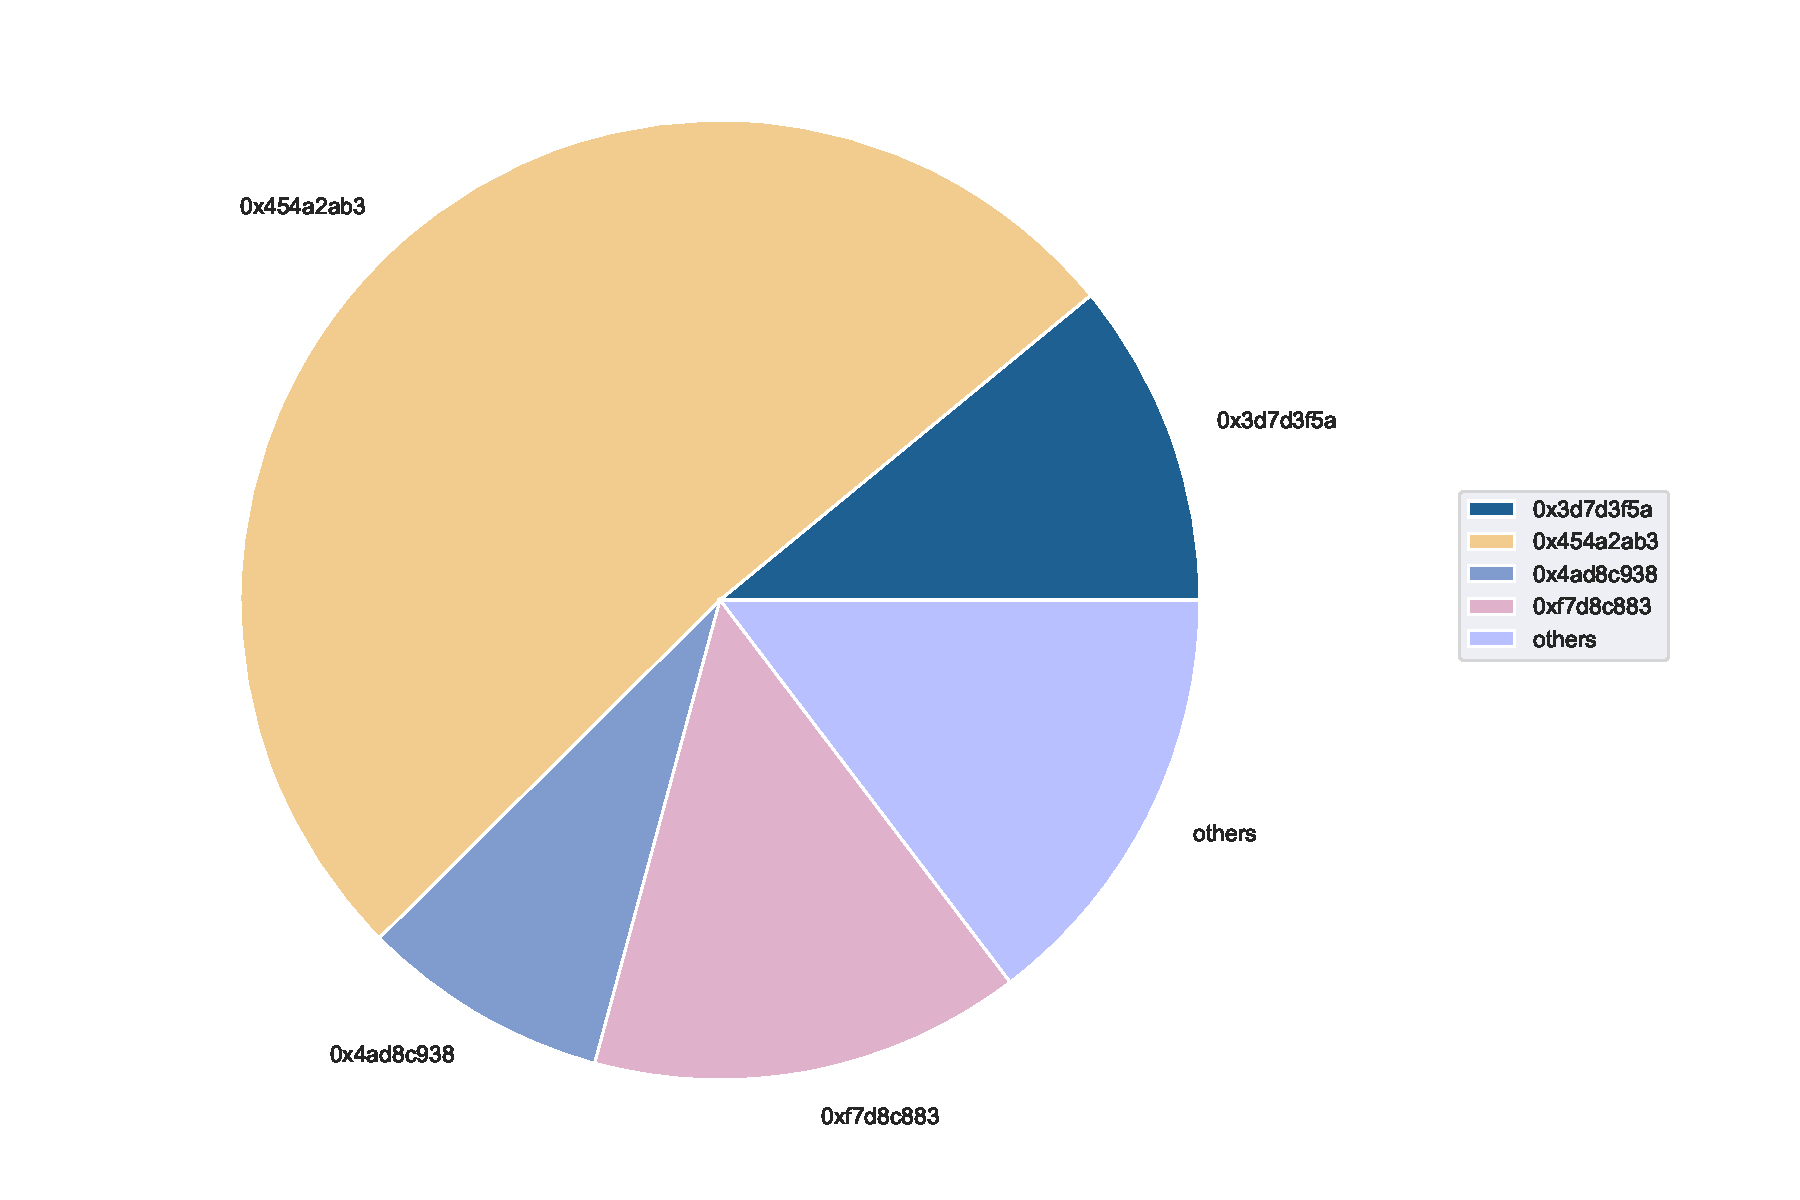
\includegraphics[height=2in]{figure/user count function1.pdf}}
	\subfigure[9-20]{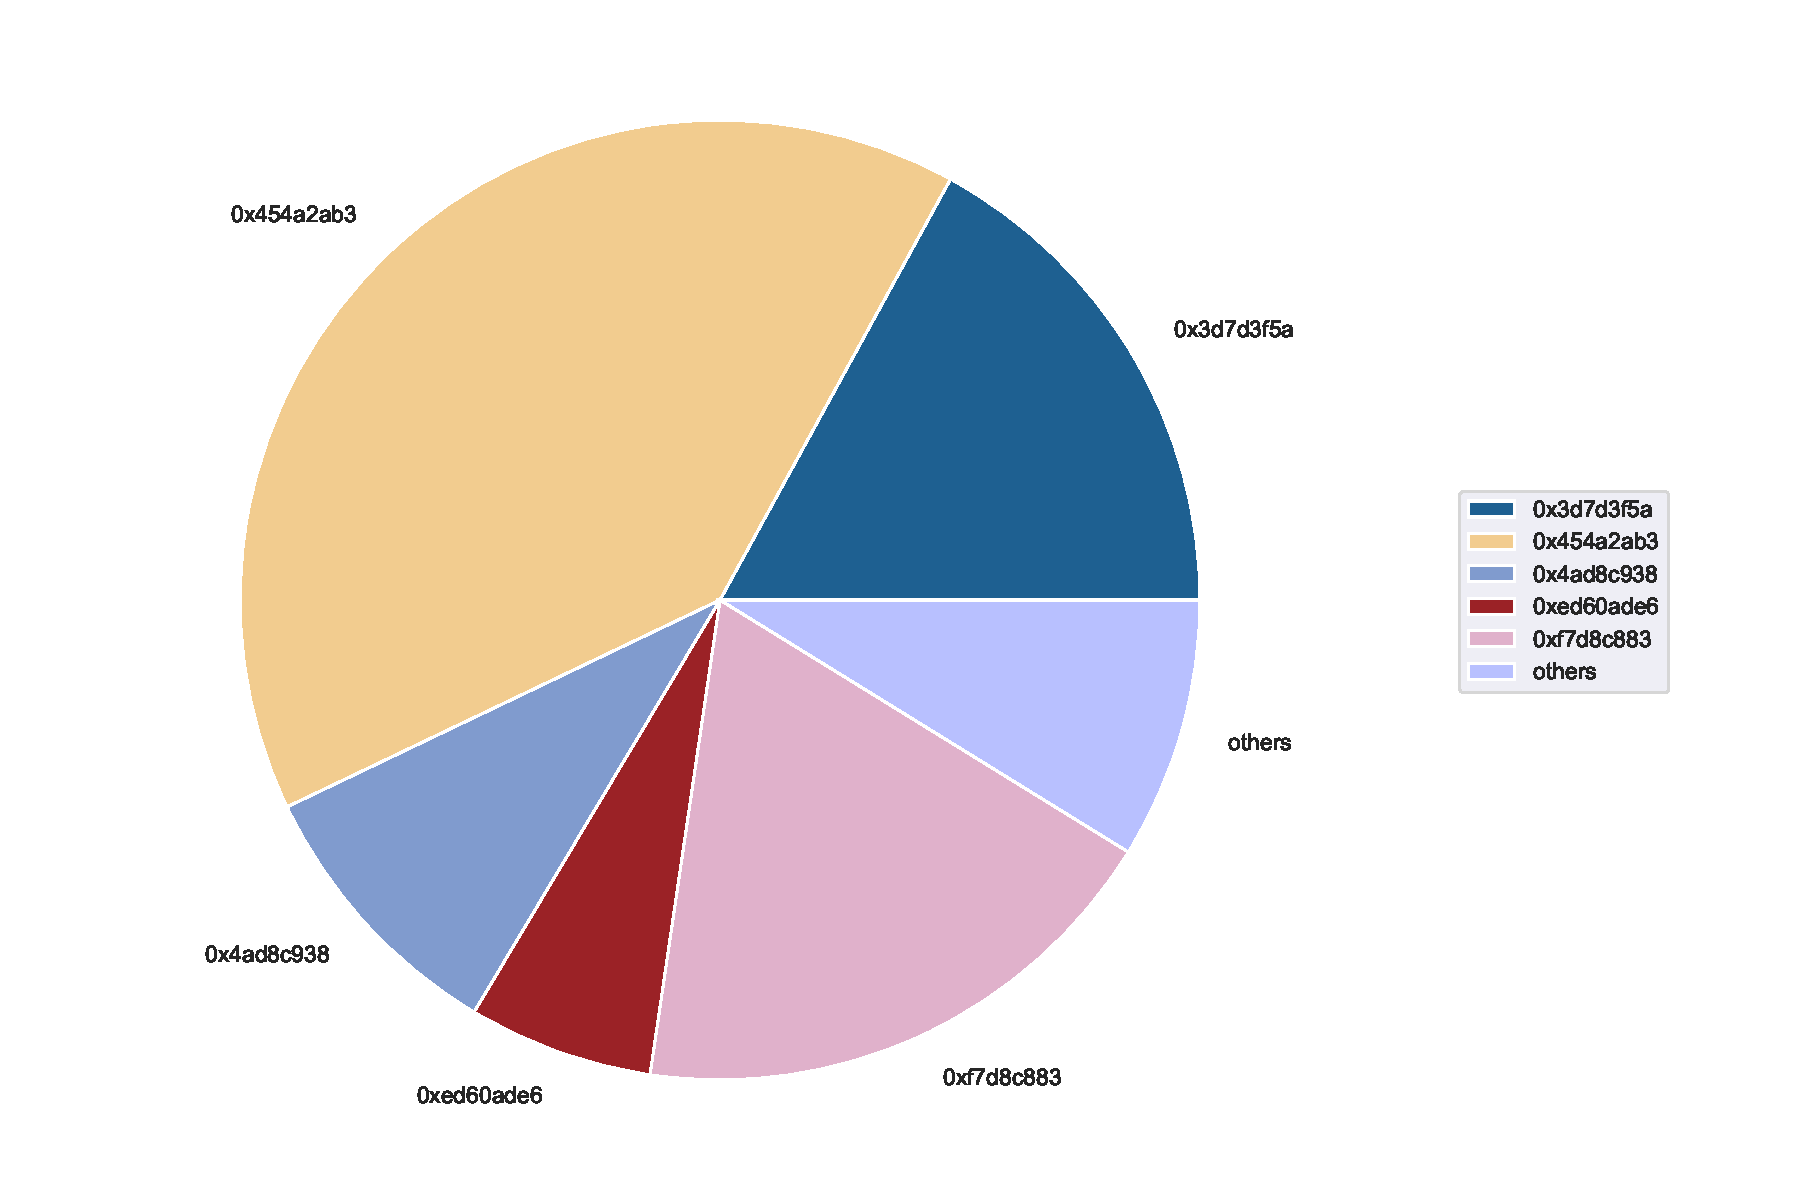
\includegraphics[height=2in]{figure/user count function2.pdf}}
	\subfigure[21-55]{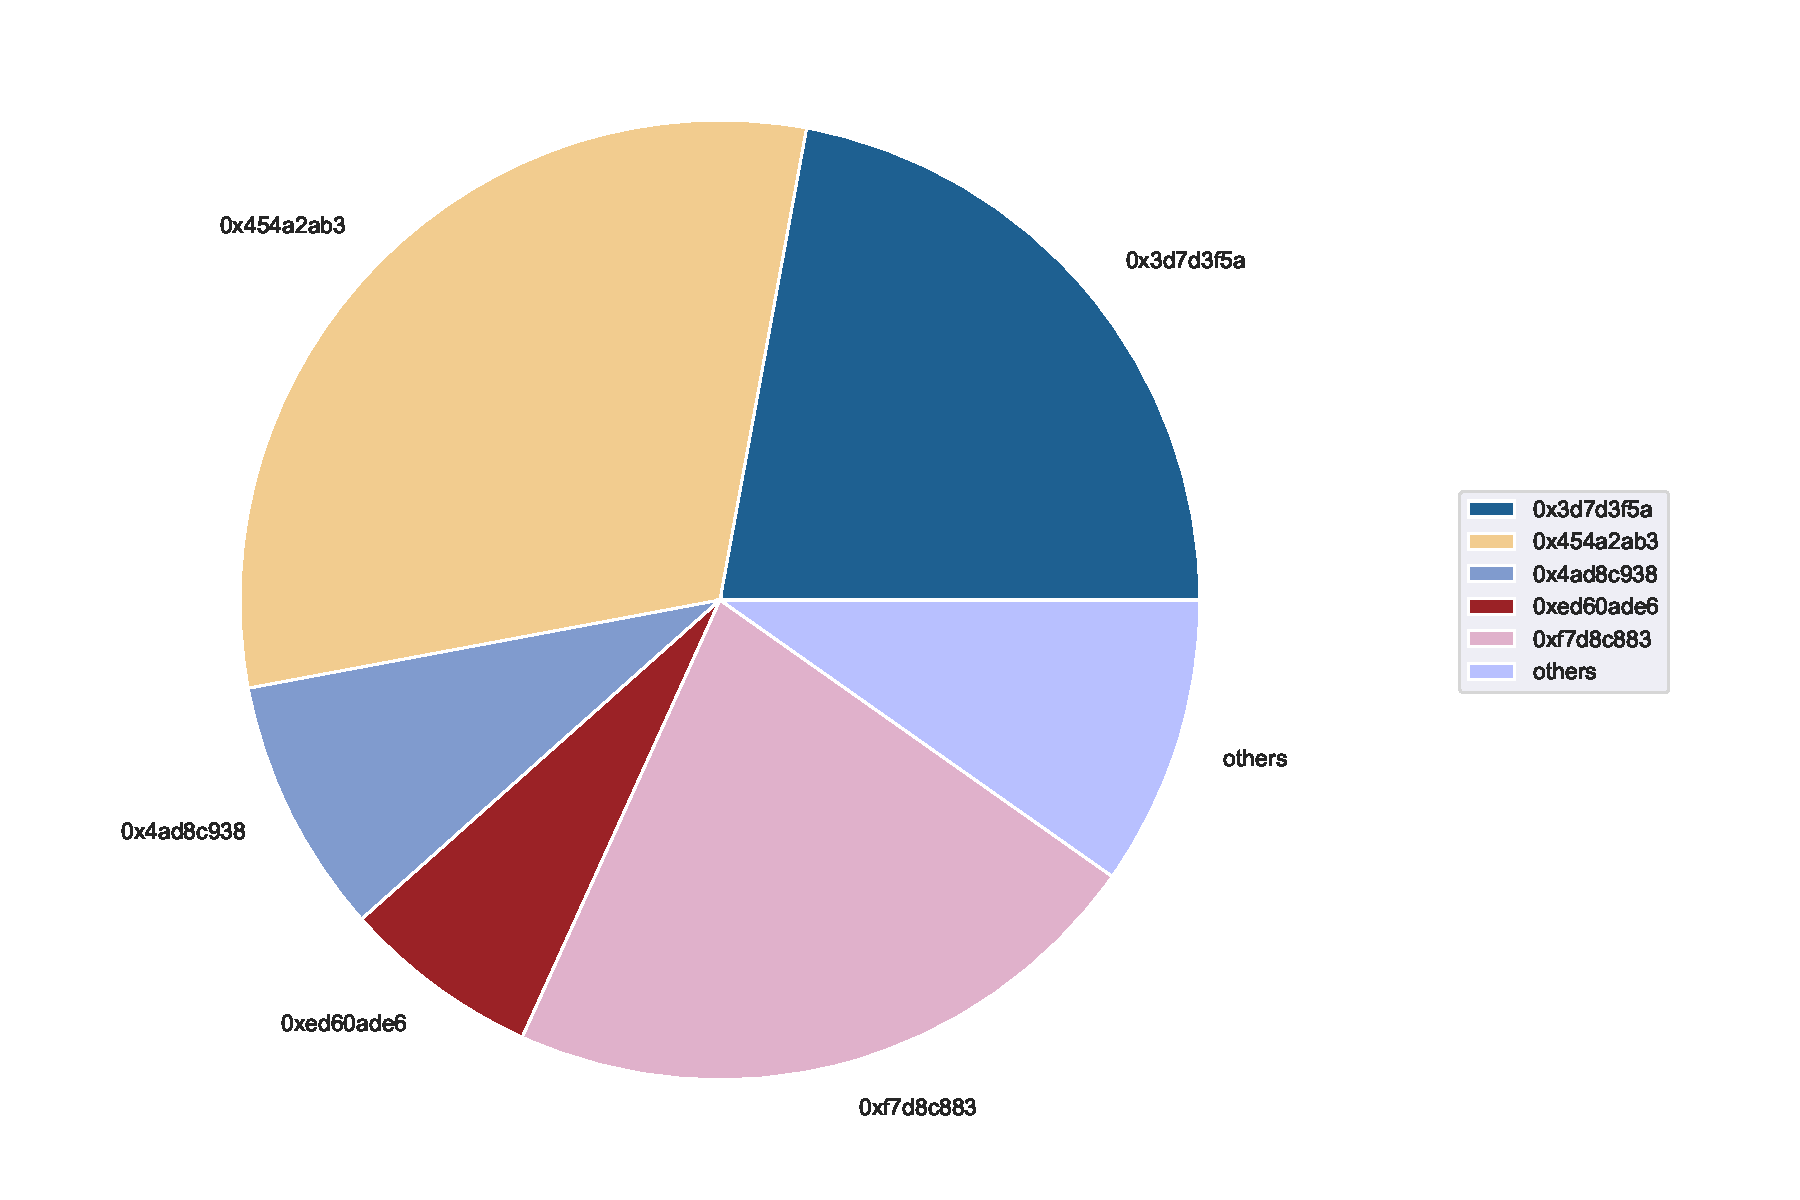
\includegraphics[height=2in]{figure/user count function3.pdf}}
	\subfigure[>55]{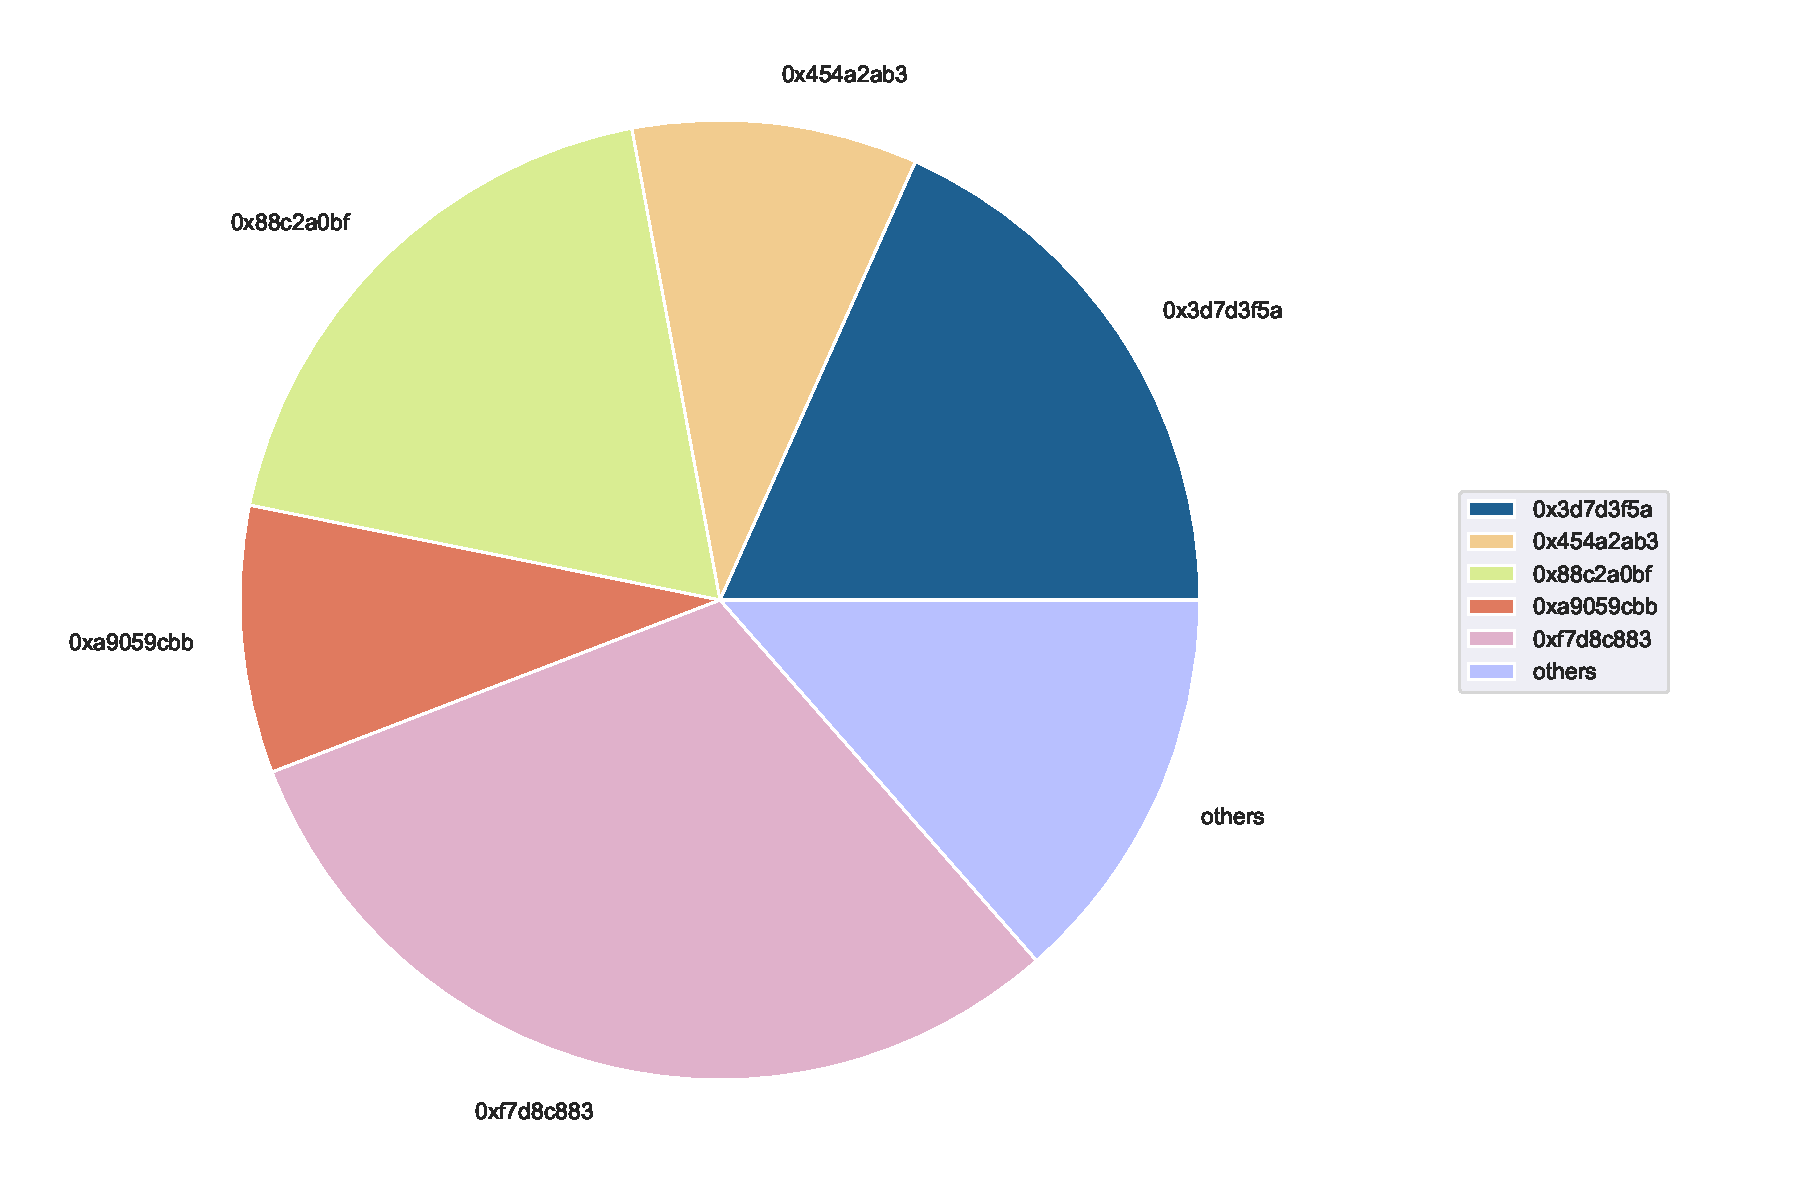
\includegraphics[height=2in]{figure/user count function4.pdf}}
	\caption{不同调用次数区间的用户调用函数的比例}
	\label{fig:user count function}
\end{figure}


\subsection{CryptoKitties的用户行为分析}
用户行为分析指的是通过对用户在使用产品和服务时的行为进行研究和分析,来了解用户的需求和行为。

在本节中,我们选取了地址为0x85a2\_9ad3\footnote{完整地址:0x85a243ceb8539884f0aa935408256c7f37c79ad3}的用户进行分析,该用户在2017年至2023年间总共调用了1497次Core和SaleAuction上的函数。在本节,我们尝试回答五个问题:
\begin{enumerate}
\item 该用户购买了哪些猫?
\item 该用户购买了哪些猫的交配权?
\item 该用户创建了哪些拍卖?
\item 该用户创建的哪些拍卖成功了?
\item 该用户自己的猫之间是如何繁衍的?
\end{enumerate}

图\ref{fig:network1}和图\ref{fig:network2}展示了该用户的行为模式图,其中绿色节点表示以太坊账户,橙色节点表示CryptoKitties中的小猫。深蓝色箭头表示用户对猫创建一个拍卖,箭头由用户指向猫;蓝色箭头表示猫被出售给某个用户,箭头由猫指向用户,不是所有的创建拍卖都会拍卖成功。橘红色的粗箭头表示用户购入某个猫,箭头由猫指向用户;红色箭头表示购买生育权用来给用户自己的猫配种,箭头由种猫指向用户的猫;黄色箭头表示用户自己的猫之间发生交配,箭头由“父亲”指向“母亲”。

整张图采用spring layout的布局算法。spring layout是一种基于力导向图(force-directed graph layout algorithm)布局的算法,通过将节点视为物理对象,并计算它们之间的斥力和吸引力来生成图形布局。其中距离越近的点表明其关系越紧密,距离越远的点表明其关系越稀疏。
\begin{figure}[!htbp]
	\centering
	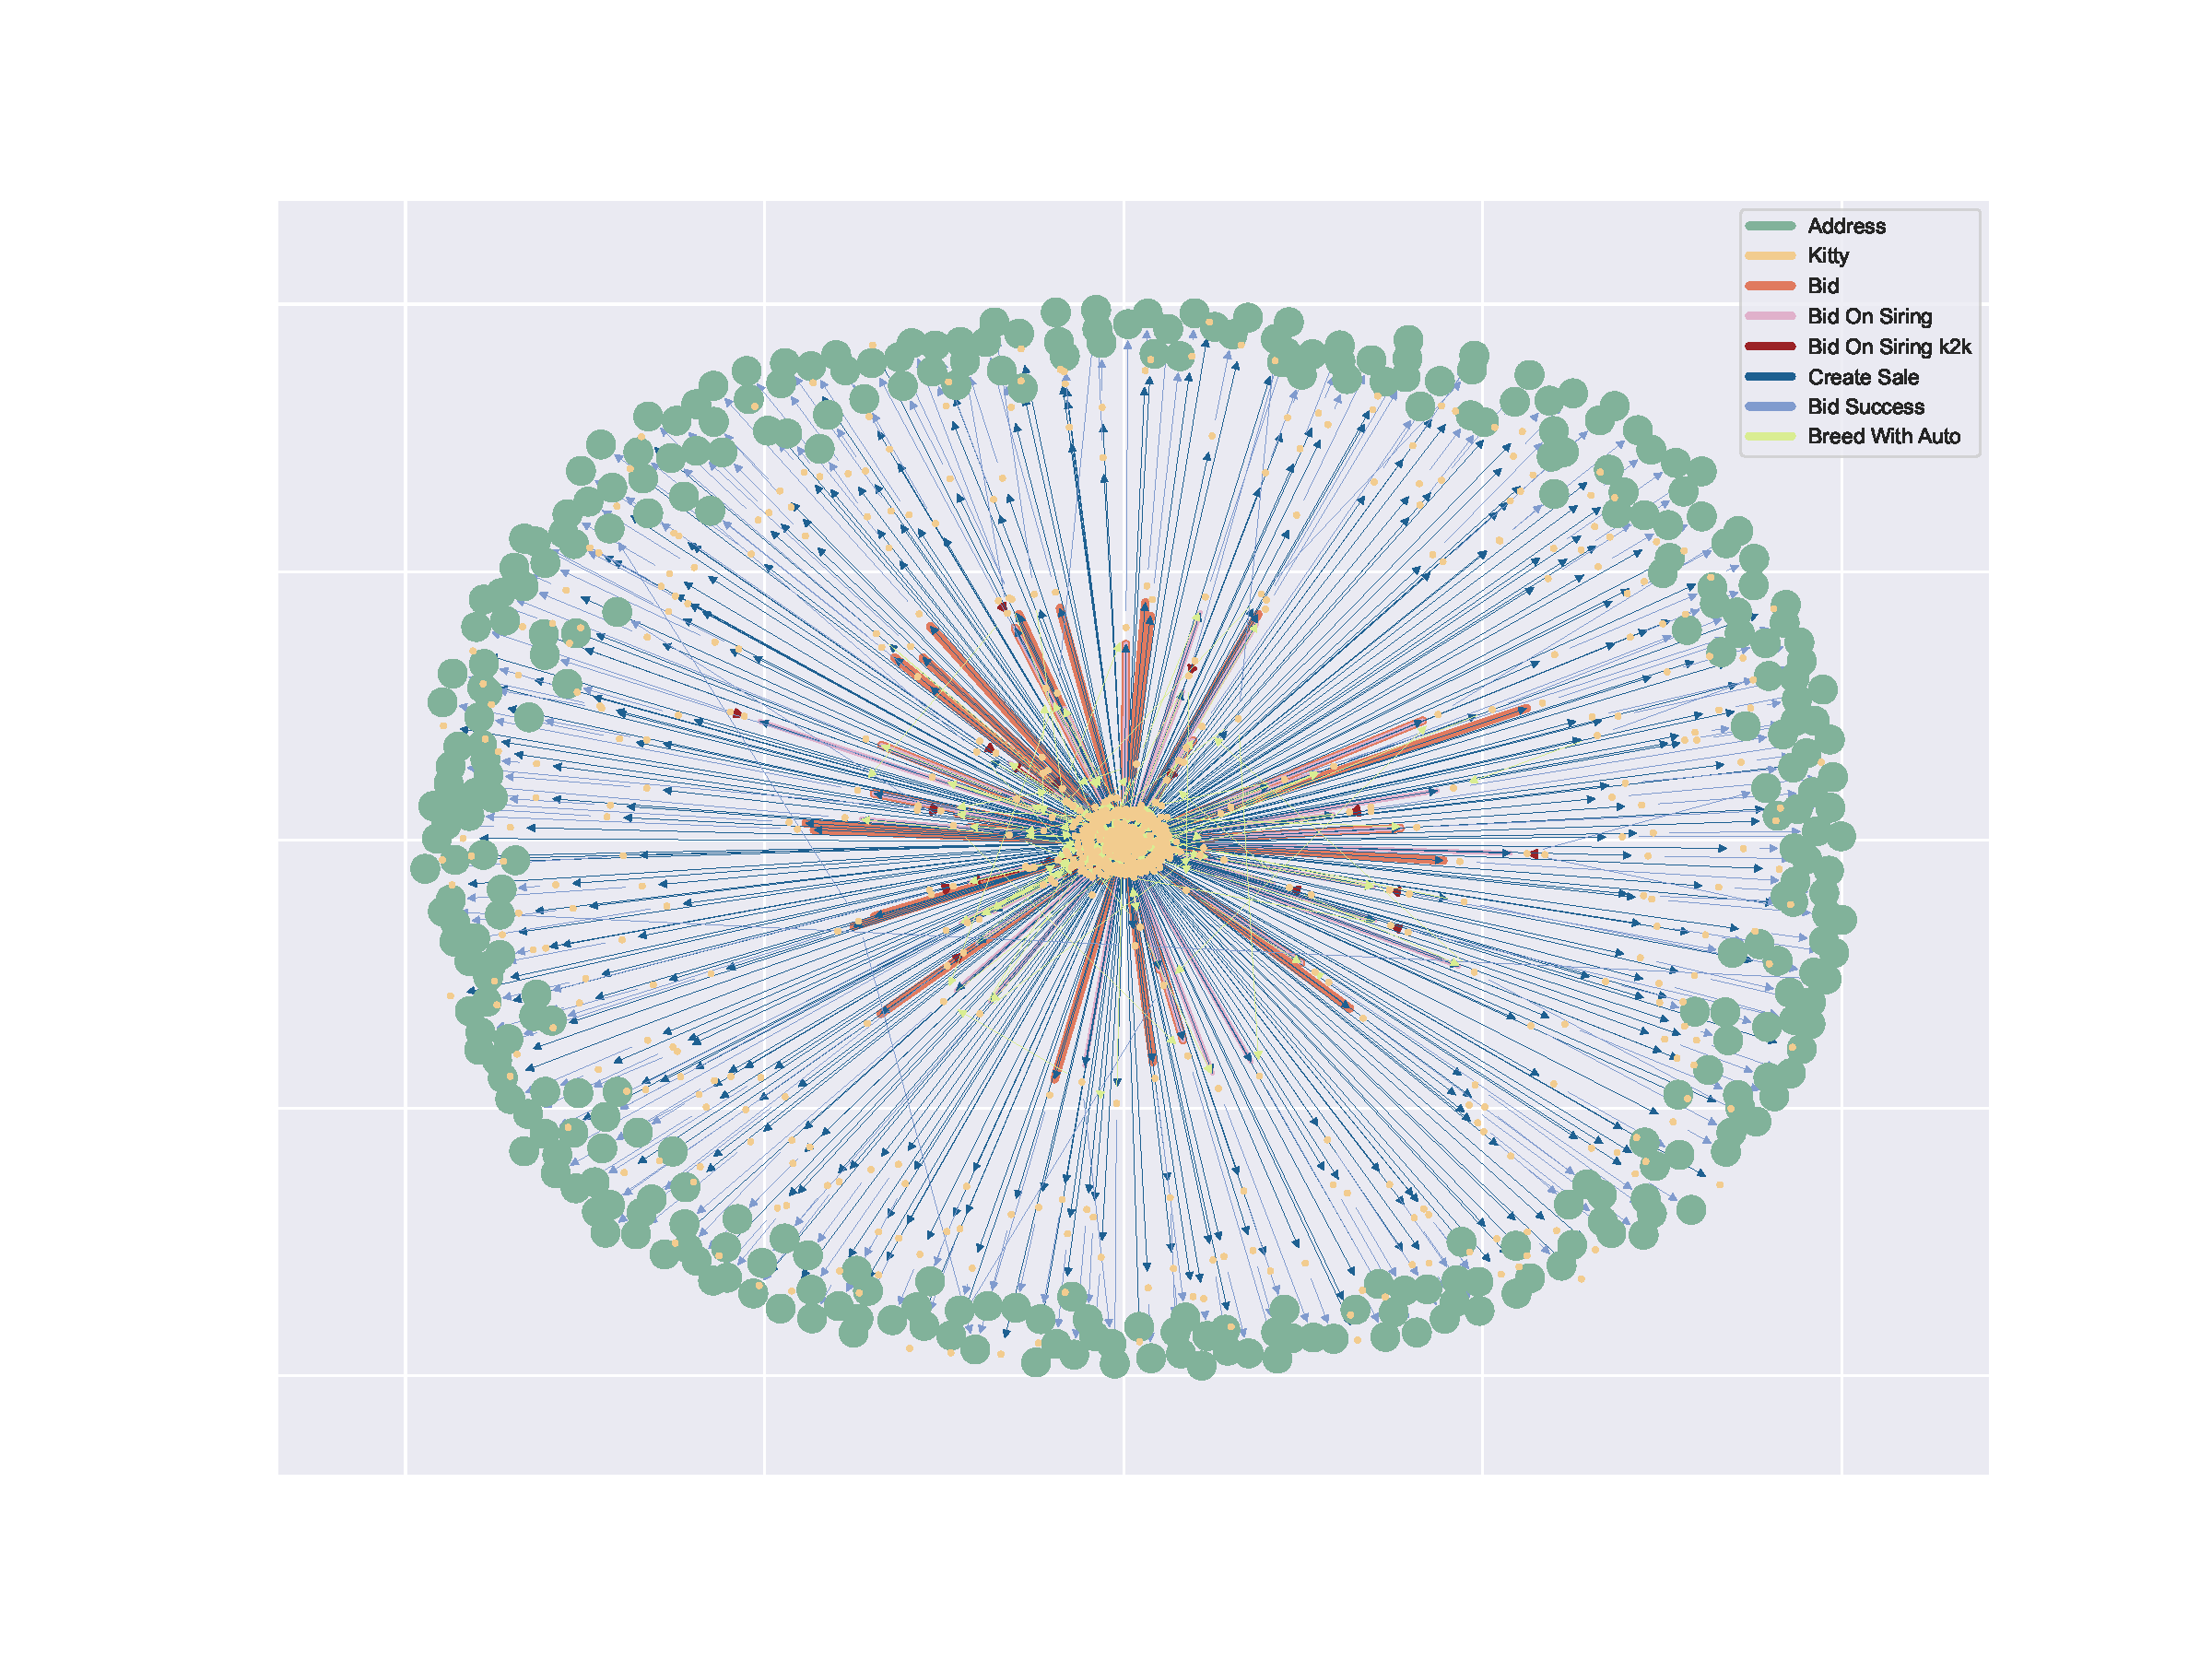
\includegraphics[width=4.5in]{figure/network1.pdf}
	\caption{用户行为模式分析}
	\label{fig:network1}
\end{figure}

\begin{figure}[!htbp]
	\centering
	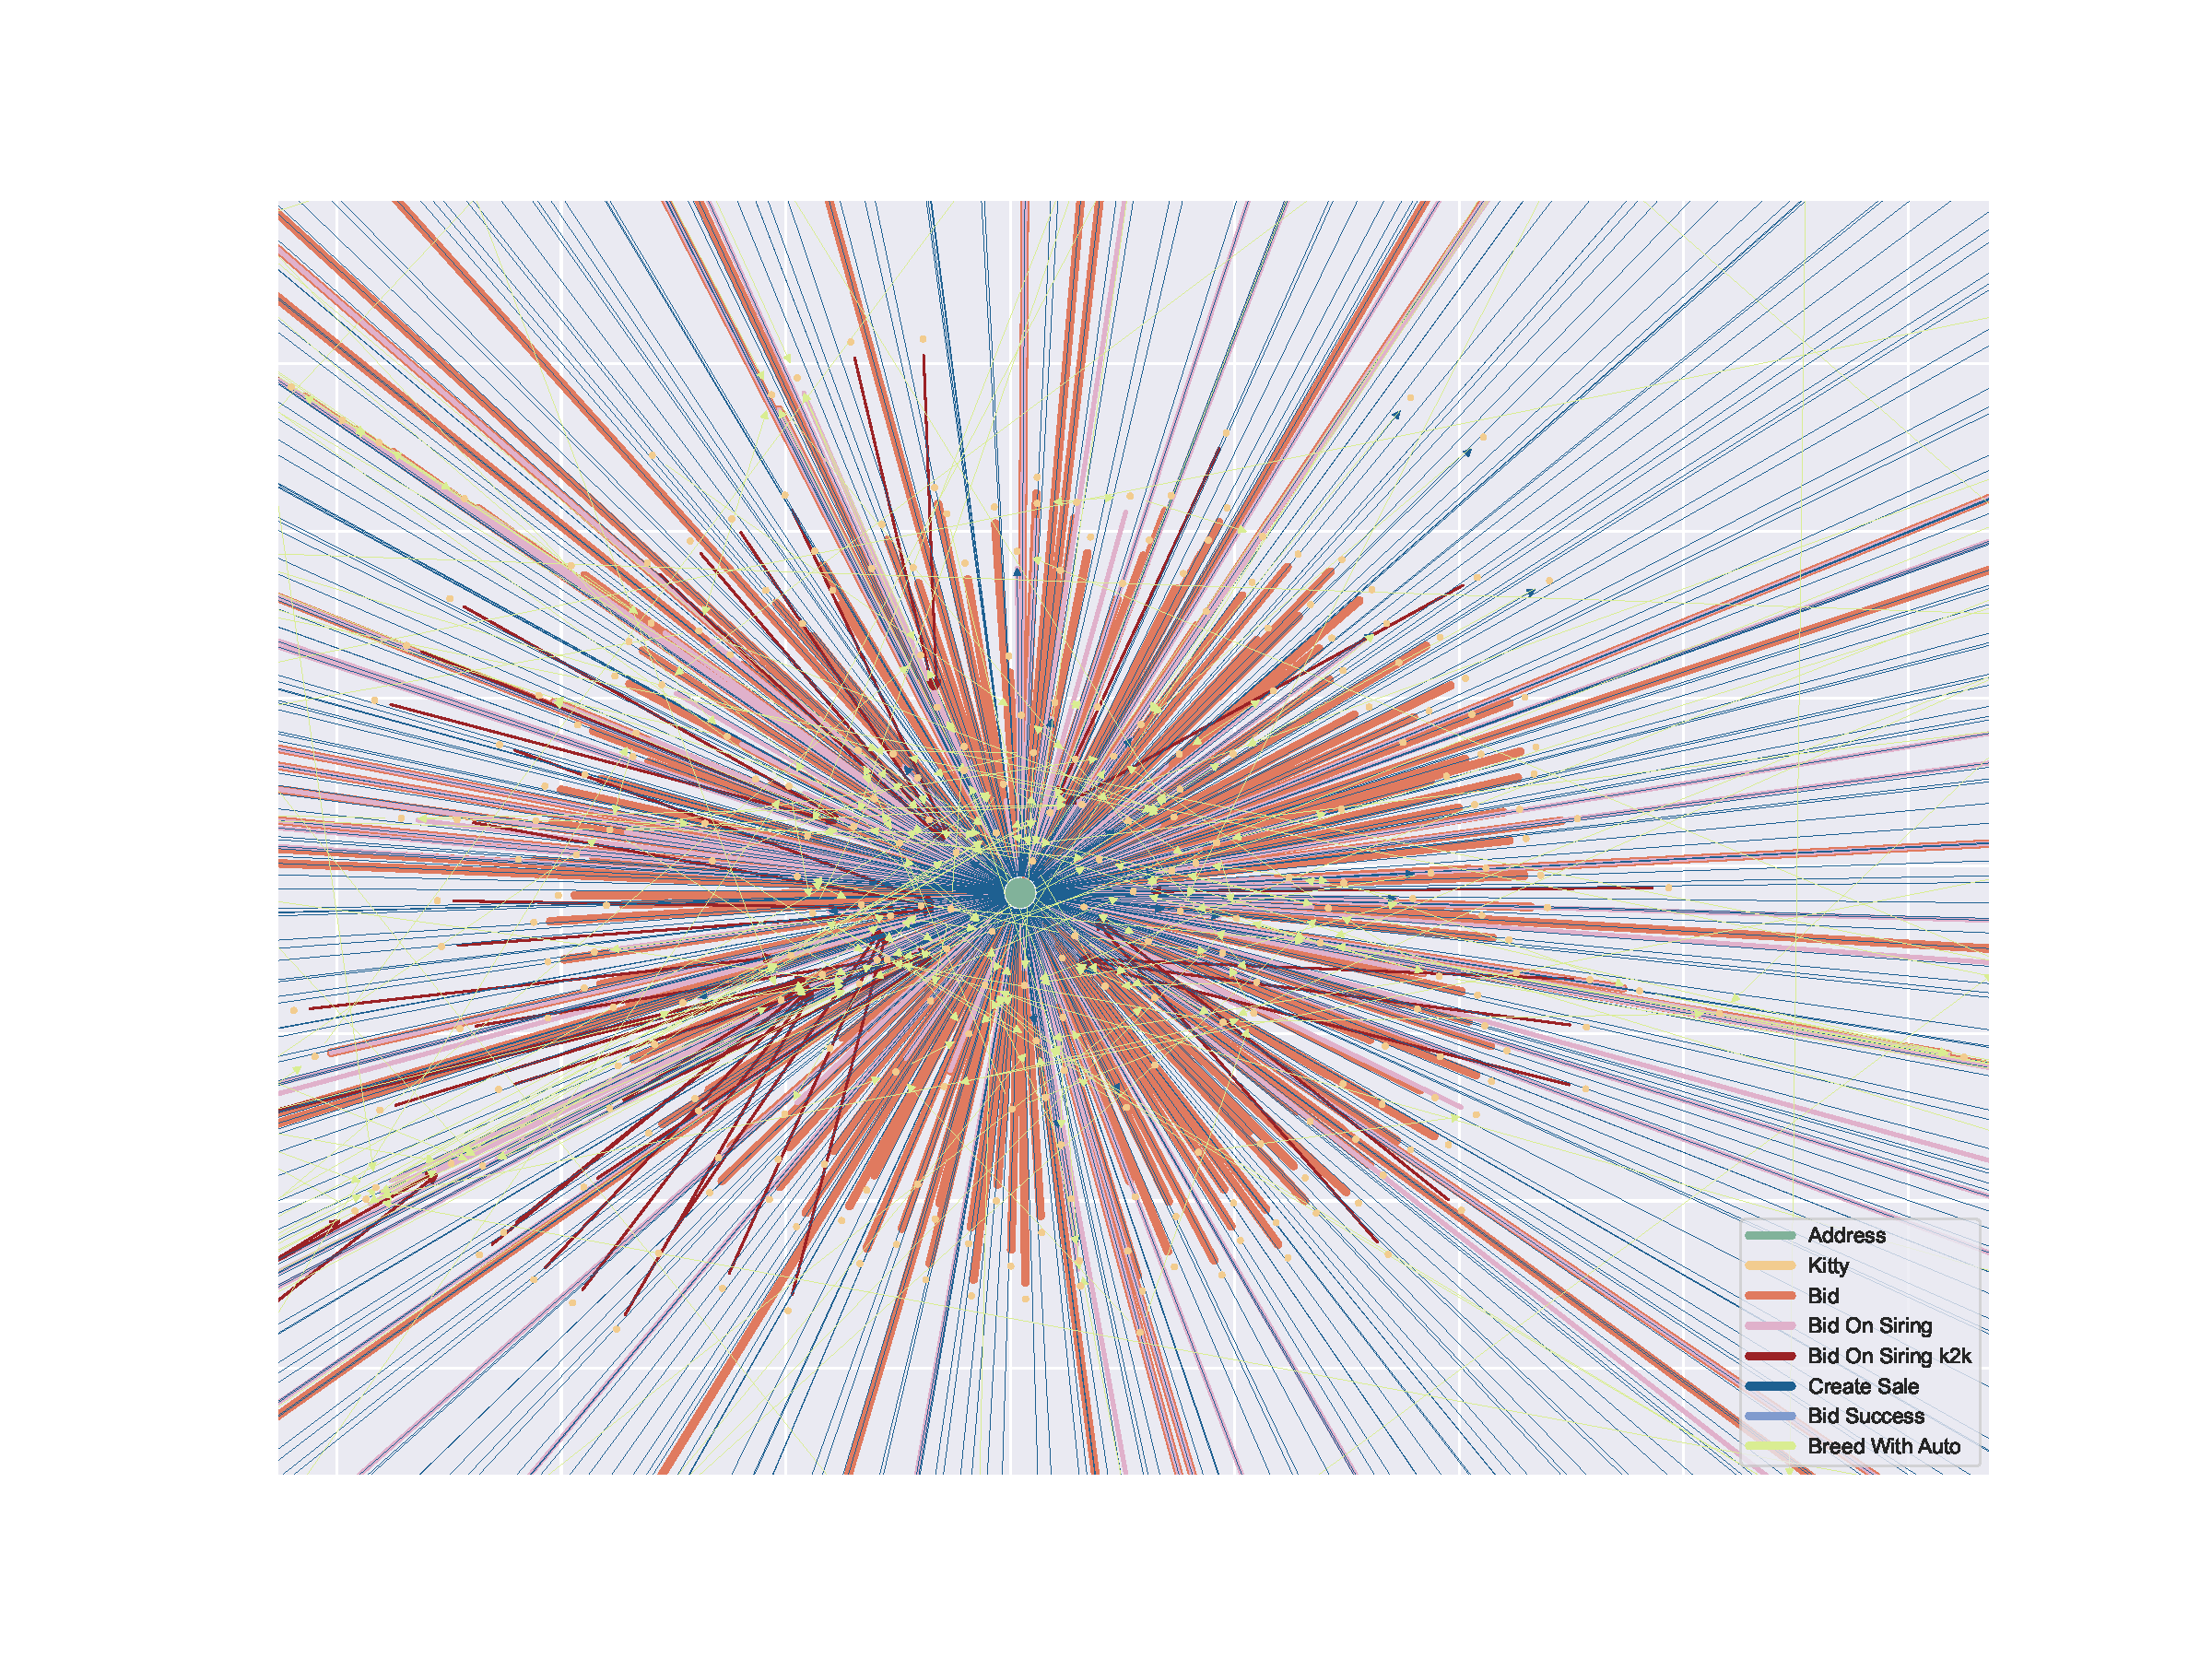
\includegraphics[width=4.5in]{figure/network2.pdf}
	\caption{用户行为模式分析}
	\label{fig:network2}
\end{figure}

图\ref{fig:network1}中中心较为密集的点关系比较“亲密”,往往与其它节点有着多种关系,如购买、生育、发起拍卖、拍卖成功等等。而外圈与以红色箭头指向中心的节点大部分只有购买和拍卖量两种关系。最外圈的节点则不存在购买关系,只存在拍卖关系和拍卖成功关系。

图\ref{fig:network2}中可以看到中心部分的详细关系。用户买入小猫,并让自己的小猫相互之间进行大量繁殖,同时也购买一定的生育权以获得更好的基因。在繁殖之后,生成的小猫被用户拿去售卖,480次拍卖中拍卖成功了434次,有较为可观的成功率与收入。

总的来说,交易频次高的用户通过购买初代猫或其它优质的猫获得原始资本,并通过繁殖产生新的小猫。一只小猫的价格一般在0.05ETH左右,而产生小猫需要使用10万左右的gas,约合0.002ETH。期间的差价即为用户的盈利。在以太坊发布完所有的初代猫以后,手握大量猫的用户就成为了新的“发行商”。如果CryptoKitties的市场不断扩大,则会有大量用户涌入并购买一只或多只小猫,卖出去的猫越多,用户的盈利就越高;而如果市场发展不佳,则有可能造成入不敷出的局面。




% \begin{figure}[!htbp]
% 	\centering
% 	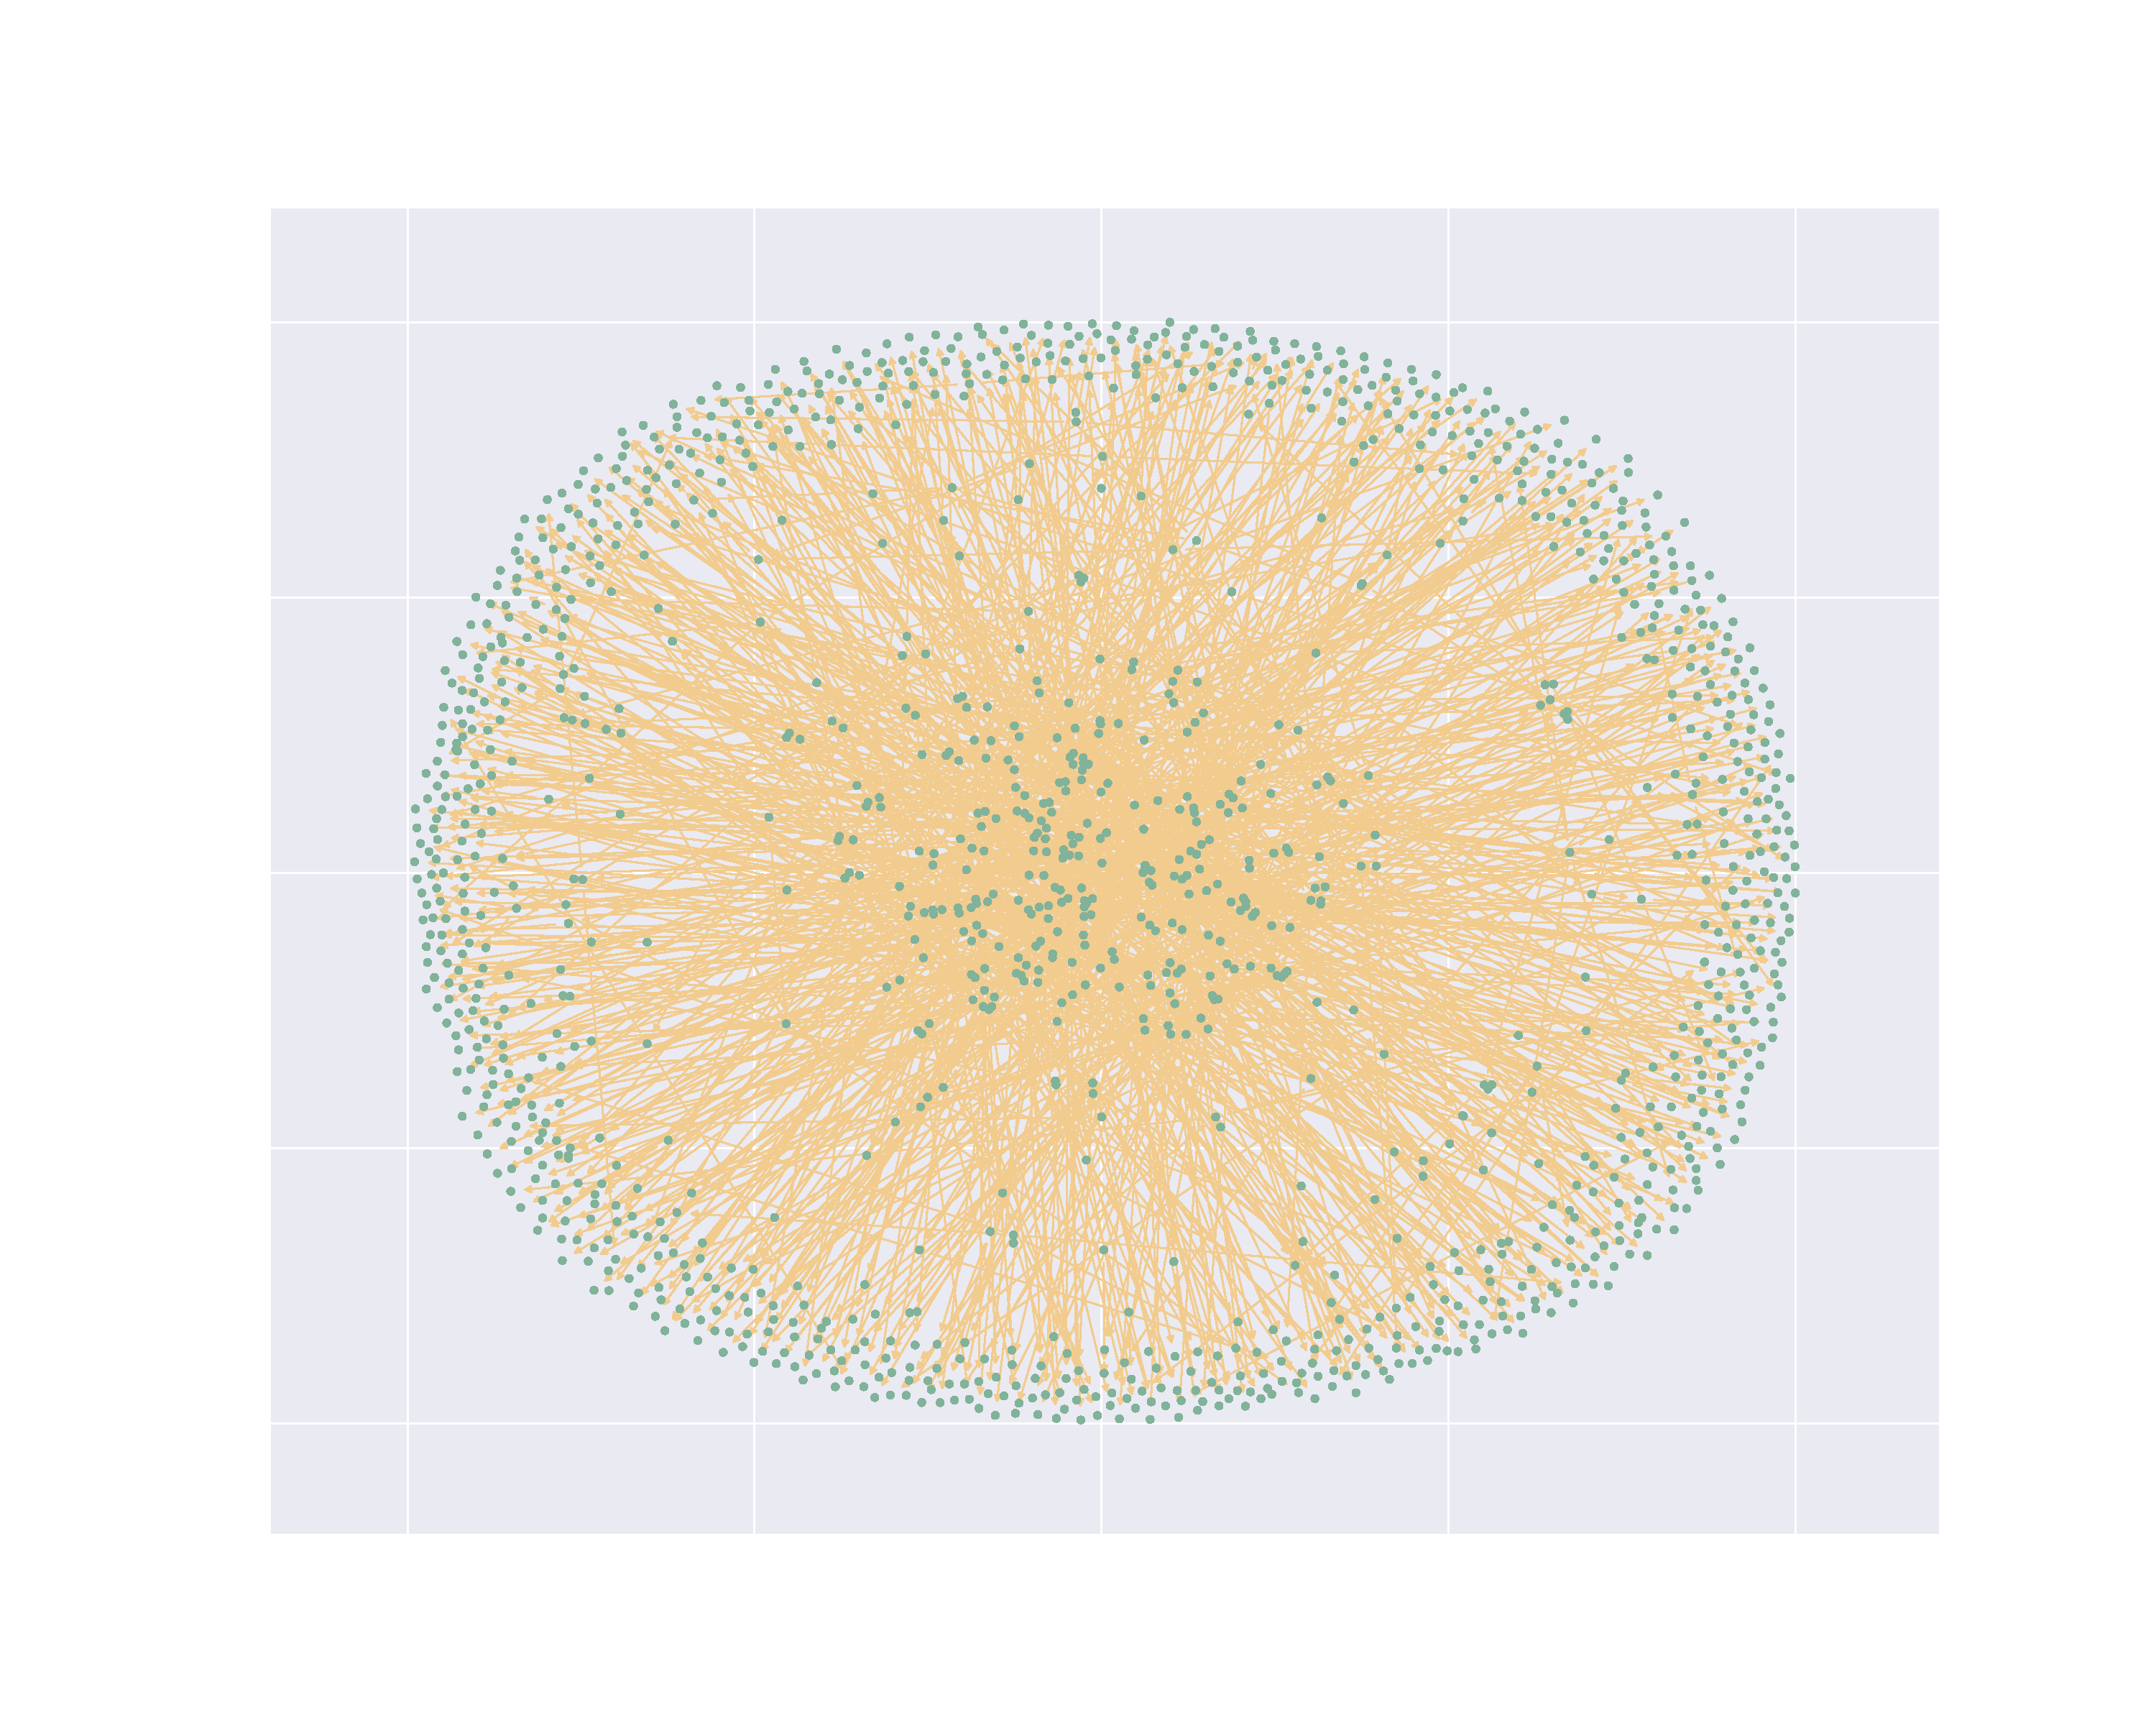
\includegraphics[width=\linewidth]{figure/cat relationship.pdf}
% 	\caption{Caption.}
% 	\label{fig:label}
% \end{figure}

\subsection{CryptoKitties中的猫的价格预测}

CryptoKitties市场中,猫的交易价格是一个非常重要的因素,它受到多种因素的影响,如稀有度、基因组合、出生日期等,在本节中,我们选取了2018年一整年的交易数据,共计292829条,通过机器学习和数据挖掘技术,对猫的交易价格进行预测。

该预测结果可以帮助CryptoKitties的玩家和投资者更好地了解市场行情,以制定合适的拍卖开始价格和结束价格。


\subsubsection{数据预处理}

\noindent \textbf{生成猫的信息}


猫的出生有两种形式:一种是CryptoKitties官方所创建的初代猫,COO每隔15分钟调用createGen0Auction函数产生一个0代的猫,并进行拍卖。另一种则是用户通过交配、怀孕,最后通过giveBirth函数生成一只新的小猫。这两种情况都会产生一个名为Birth的Event Log,其中记录了新出生的猫的所有者、Id、母亲的Id、父亲的Id和这只猫的基因。从这些数据中,我们可以获取到每只猫的基因、猫的代数以及每只猫每次繁衍的时间。

其中,猫的代数为其父亲的代数和母亲的代数的最大值加一,即
\begin{align*}
{\rm kitty\_generation} = \max({\rm matron\_generation},{\rm sire\_generation})+1
\end{align*}
猫的代数影响了猫生育后的休息时间,如表\ref{tab:generation}所示。此外当这只猫繁衍后,它的特征会发生变化。每次繁衍等同于增加了一个代。如果一只3代猫繁衍了3次,它的修养特征会变成第6代的Snappy。这样就限制了一只猫的繁衍速度,增加了低代的稀有价值,也限制了稀有基因的遗传效率。

\begin{table}[tb]
	\caption{不同代的猫的初始生育休息时间}
	\label{tab:generation}
	\centering

	\begin{tabular}{l|cc}
	\hline

	\hline
	\textbf{代} & \textbf{特征} & \textbf{修养时间} \\
	\hline
	0 · 1&	Fast&	1分钟\\
		\hline
	2 · 3&	Swift&	2分钟\\
		\hline
	4 · 5&	Swift&	5分钟\\
		\hline
	6 · 7&	Snappy&	10分钟\\
		\hline
	8 · 9&	Snappy&	30分钟\\
		\hline
	10 · 11&	Brisk&	1小时\\
		\hline
	12 · 13&	Brisk&	2小时\\
		\hline
	14 · 15&	Plodding&	4小时\\
		\hline
	16 · 17&	Plodding&	8小时\\
		\hline
	18 · 19&	Slow&	16小时\\
		\hline
	20 · 21&	Slow&	24小时\\
		\hline
	22 · 23&	Sluggish&	2天\\
		\hline
	24 · 45&	Sluggish&	4天\\
		\hline
	26+&	Catatonic&	1周\\

	\hline
	\end{tabular}
\end{table}


猫的基因由一个64位的16进制数表示,将其转换成256的2进制数后,去掉前16位的0,剩余240位,每5位为一组,对应了48个基因位,用Kai编码表示。48个基因位中每4个位一组,形成12块,如图\ref{fig:gene}所示。在每一个基因块中,第四位表示了当前猫的显性性状,其它倒数第二位、第三位、第四位分别表示了第一、第二、第三隐性性状。

\begin{figure}[!htbp]
	\centering
	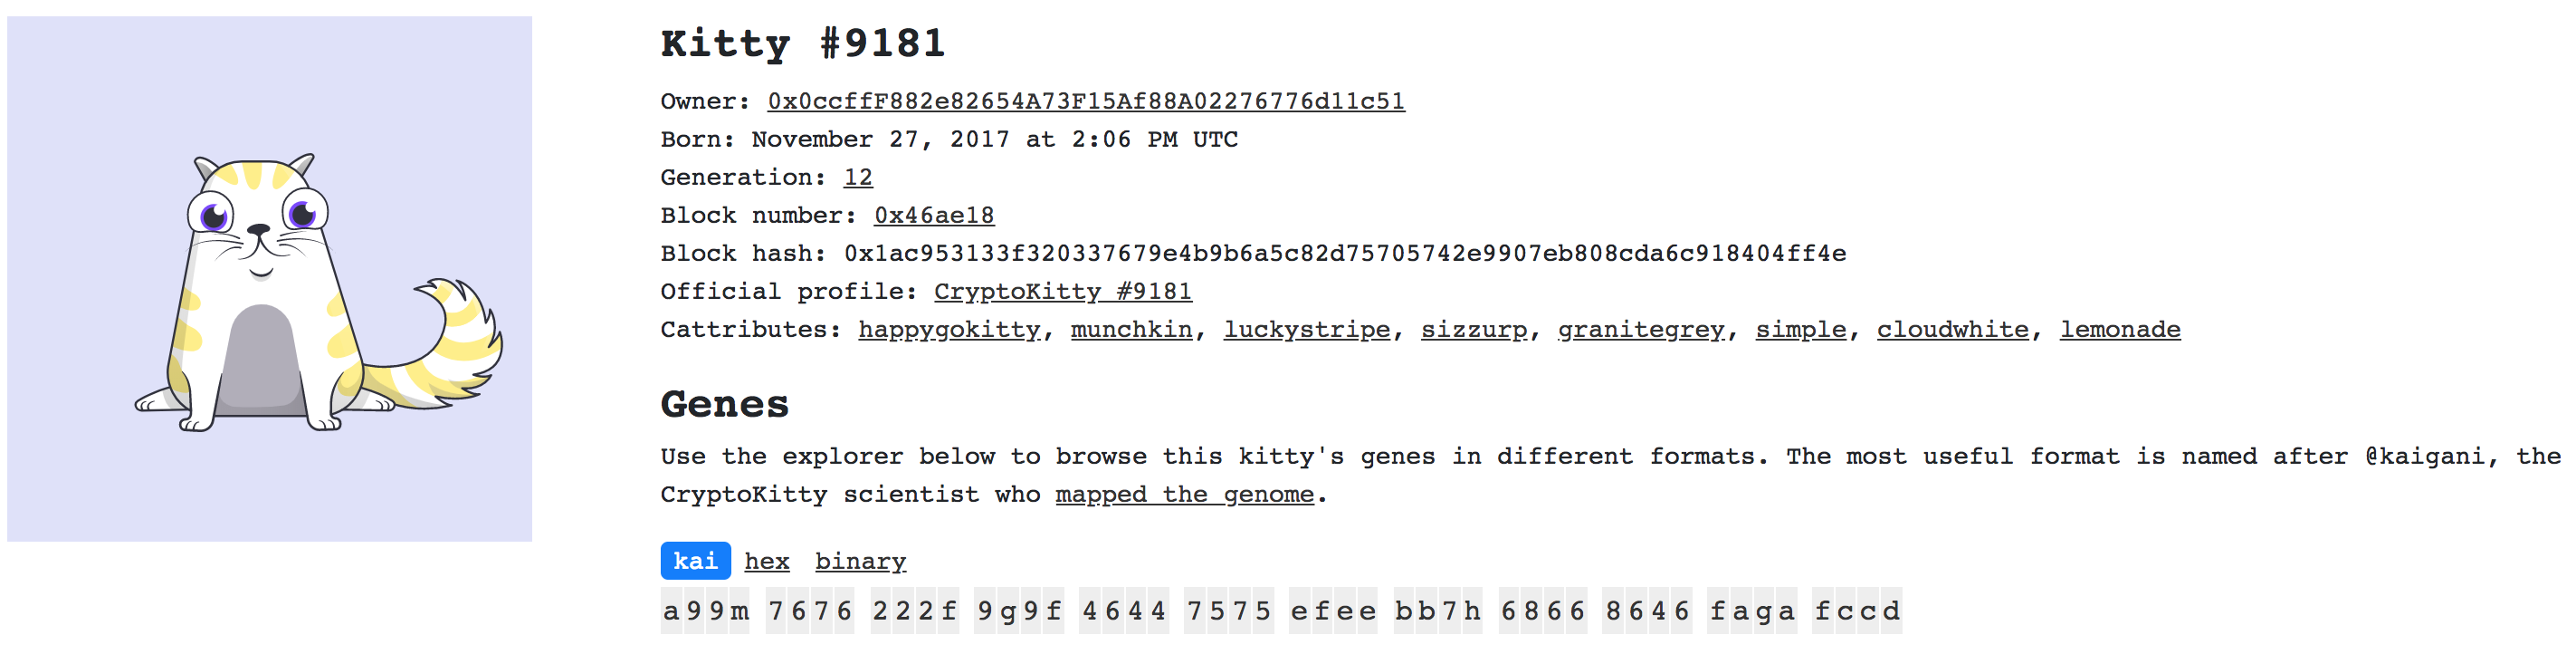
\includegraphics[width=\linewidth]{figure/gene.png}
	\caption{基因编码}
	\label{fig:gene}
\end{figure}

显然,猫的基因、代和交易前的繁衍次数都会影响其交易价格。在这一部分中,我们选取了2018年以前Log数据库中合约地址为Core且topic为Birth的所有数据(2018年的交易数据可能包含2018年以前生成的猫),通过解析log data得到kittyId、matronId、sireId、gene四个字段的信息,并获取log所在的区块的编号block\_number作为出生时间。由于每只猫只会出生一次,因此用猫的Id作为索引\footnote{加快索引速度}。随后添加pregant字段,遍历整张表,在每只小猫的母亲的pregant字段中添加小猫的出生区块号。最后添加generation字段,将初代猫初始化为第0代,通过递归的方式计算每只猫的代数。


\noindent \textbf{生成市场信息}


除了猫本身,市场的活跃度和供需关系显然也会影响到猫的市场价格。因此和研究主题一中类似的,统计每日创建销售拍卖的次数、创建生育拍卖的次数、销售拍卖成功的数量和生育拍卖成功的数量和birth和breedWithAuto的调用次数。由于供需关系(bid-createSaleAuction)是bid和createSaleAuction的线性组合,因此舍去。

\noindent \textbf{生成销售数据}


以Sale Auction中调用函数为bid的数据为基础,从input中解析出竞拍的小猫的Id,通过Id连接包含所有猫的数据的表kitty\_table。再通过日期连接市场活跃度的表market,和以太币价格的表price,从而得到sale\_data。

遍历sale\_data,对于每个竞拍成功的数据,从Core中通过kittyId找到createSaleAuction的候选者,再通过日期的关系找到bid对应的createSaleAuction。并获取其初始价格、结束价格和持续时间。

最后通过猫的pregent的区块编号列表和bid时的区块编号计算在拍卖之前,该猫一共生育过所少次。并将48位kai编码的基因序列转换为48个类别变量,并保存。


\noindent \textbf{变量筛选与变量处理}


\begin{enumerate}
\item 计算以美元结算的交易价格。
\item 删除所有数值变量和类别变量以外的变量,如transactions\_hash、transactions\_input等等。
\item 删除与预测竞拍价格无关的变量,如transactions\_block\_number、transaction\_index、start\_price、end\_price、transactions\_value等等。
\item 将类别变量转换为独热编码。首先将48个基因位转换为独热编码,另外由于代(generation)是离散且非线性变化的,因此代也作为类别变量被转换为独热编码。
\item 将左偏的数据进行对数化处理,使数据分布更加接近正态分布,更符合线性回归的假设。所有数值数据的分布情况如图\ref{fig:variable distribution}所示。可以看到,竞拍价格(bid price)、持续时间(duration)、生育次数(pregnant count)、油费(gas\_price)有较为严重的左偏现象。因此对这些变量进行对数化处理。
\end{enumerate}

最终得到了共计1470个变量。

\begin{figure}[!h]
	\centering
	\subfigure[bid price]{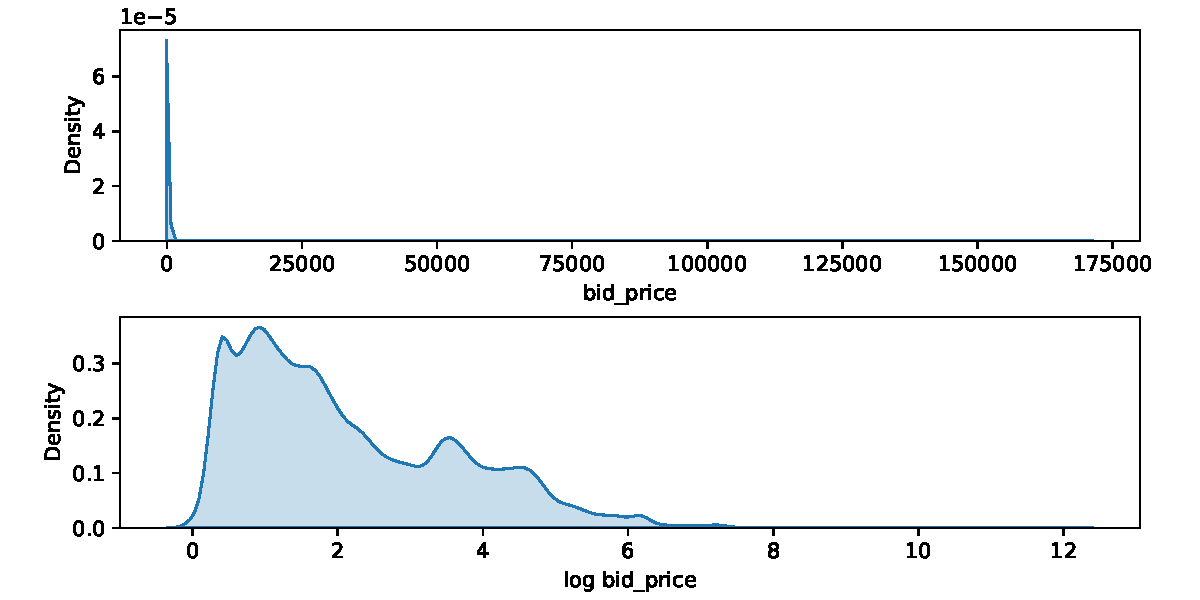
\includegraphics[height=1.5 in]{figure/variable bid_price.pdf}}
	\hspace{0 pt}
	\subfigure[duration]{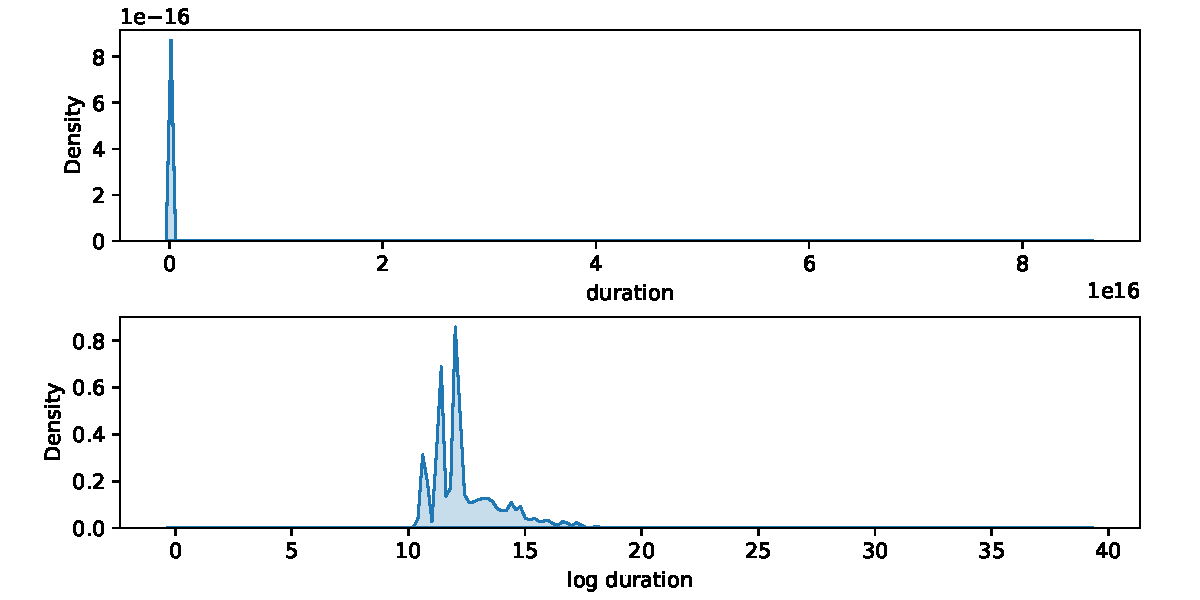
\includegraphics[height=1.5 in]{figure/variable duration.pdf}}
	\hspace{0 pt}
	\subfigure[eth price]{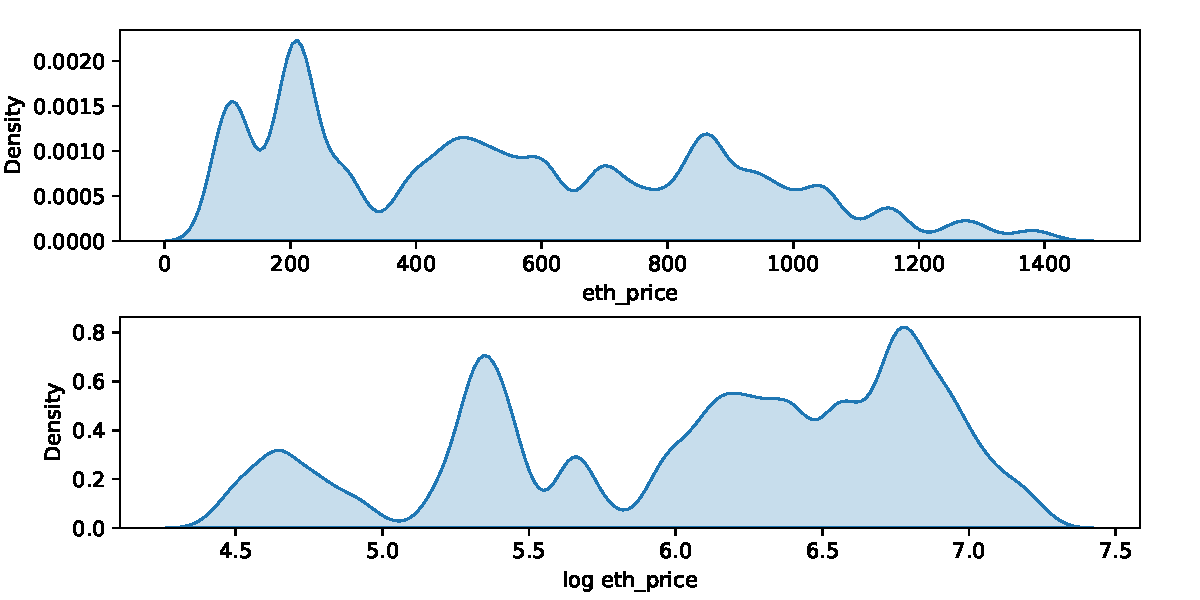
\includegraphics[height=1.5 in]{figure/variable eth_price.pdf}}
	\hspace{0 pt}
	\subfigure[pregnant count]{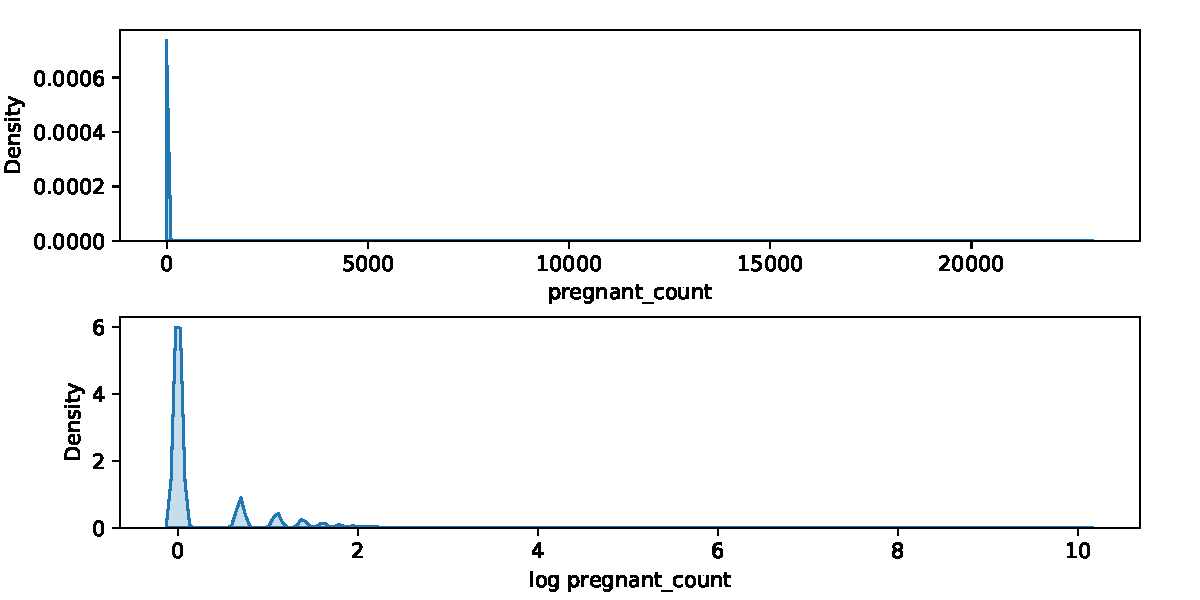
\includegraphics[height=1.5 in]{figure/variable pregnant_count.pdf}}
	\hspace{0 pt}
	\subfigure[transactions gas price]{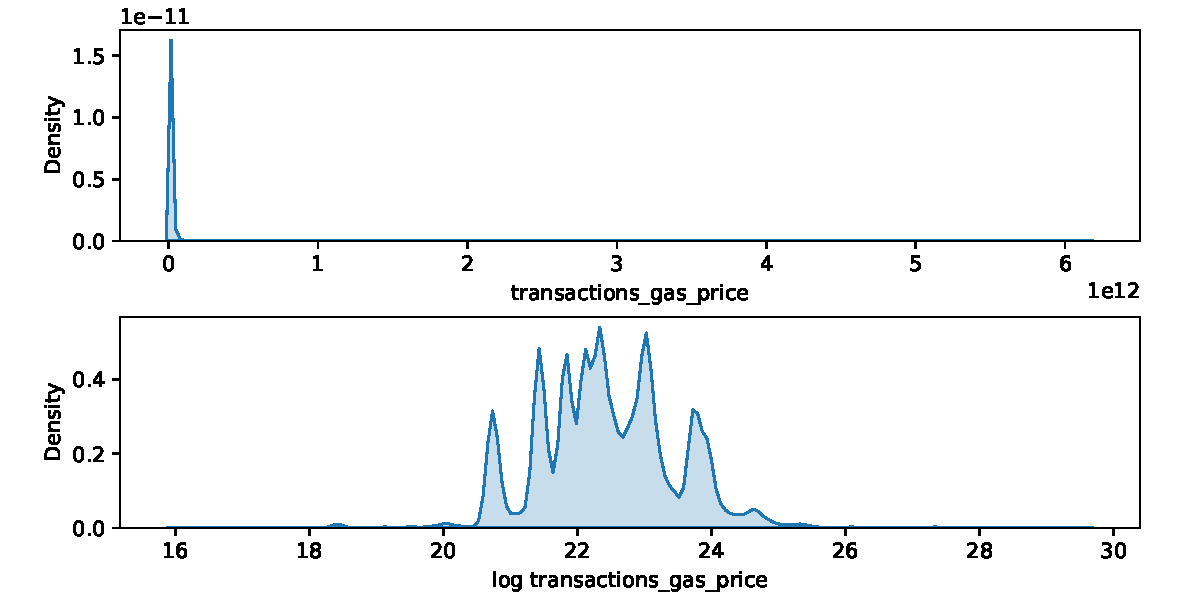
\includegraphics[height=1.5 in]{figure/variable transactions_gas_price.pdf}}
	\hspace{0 pt}
	\subfigure[eth price]{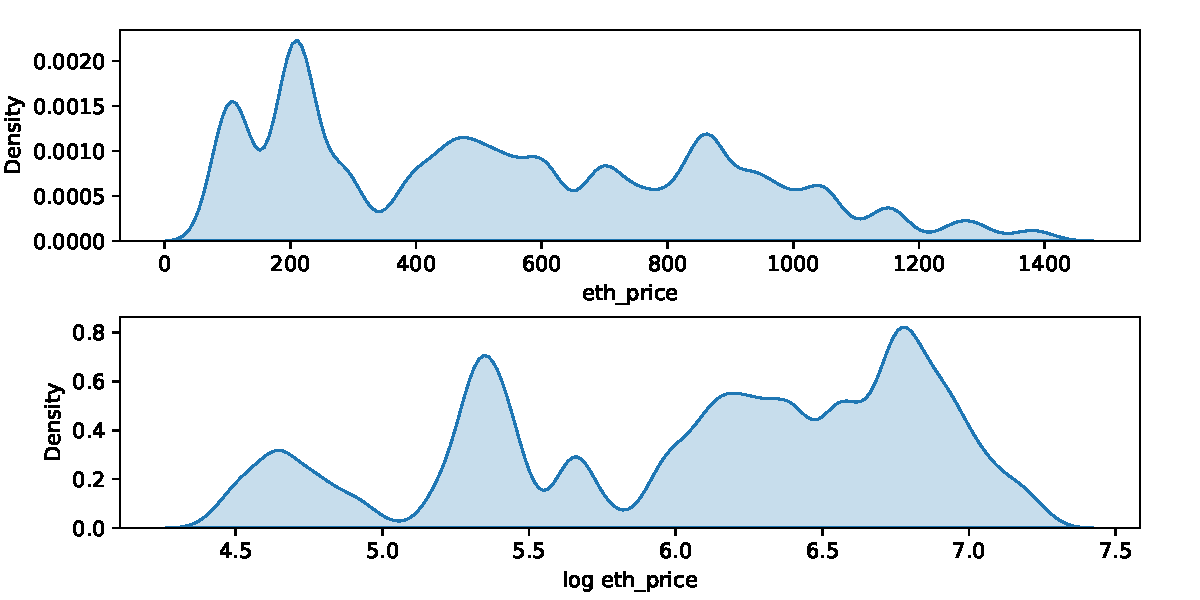
\includegraphics[height=1.5 in]{figure/variable eth_price.pdf}}

	\caption{数值变量分布}
	\label{fig:variable distribution}
\end{figure}



\subsubsection{运行结果}
经过线性回归模型的拟合后,MSE为0.664,$R^2$为0.703,可解释能力较强。

其中,价格随着交易时间、持续时间、创建销售拍卖的数量、以太币价格的增加而增加,随创建生育拍卖的数量和汽油费的增加而下降。

基因部分的系数如图\ref{fig:gene coef}所示。其中红色代表系数为正,蓝色代表系数为负。所有系数被限制在-1到1之间。

\begin{figure}[!htbp]
	\centering
	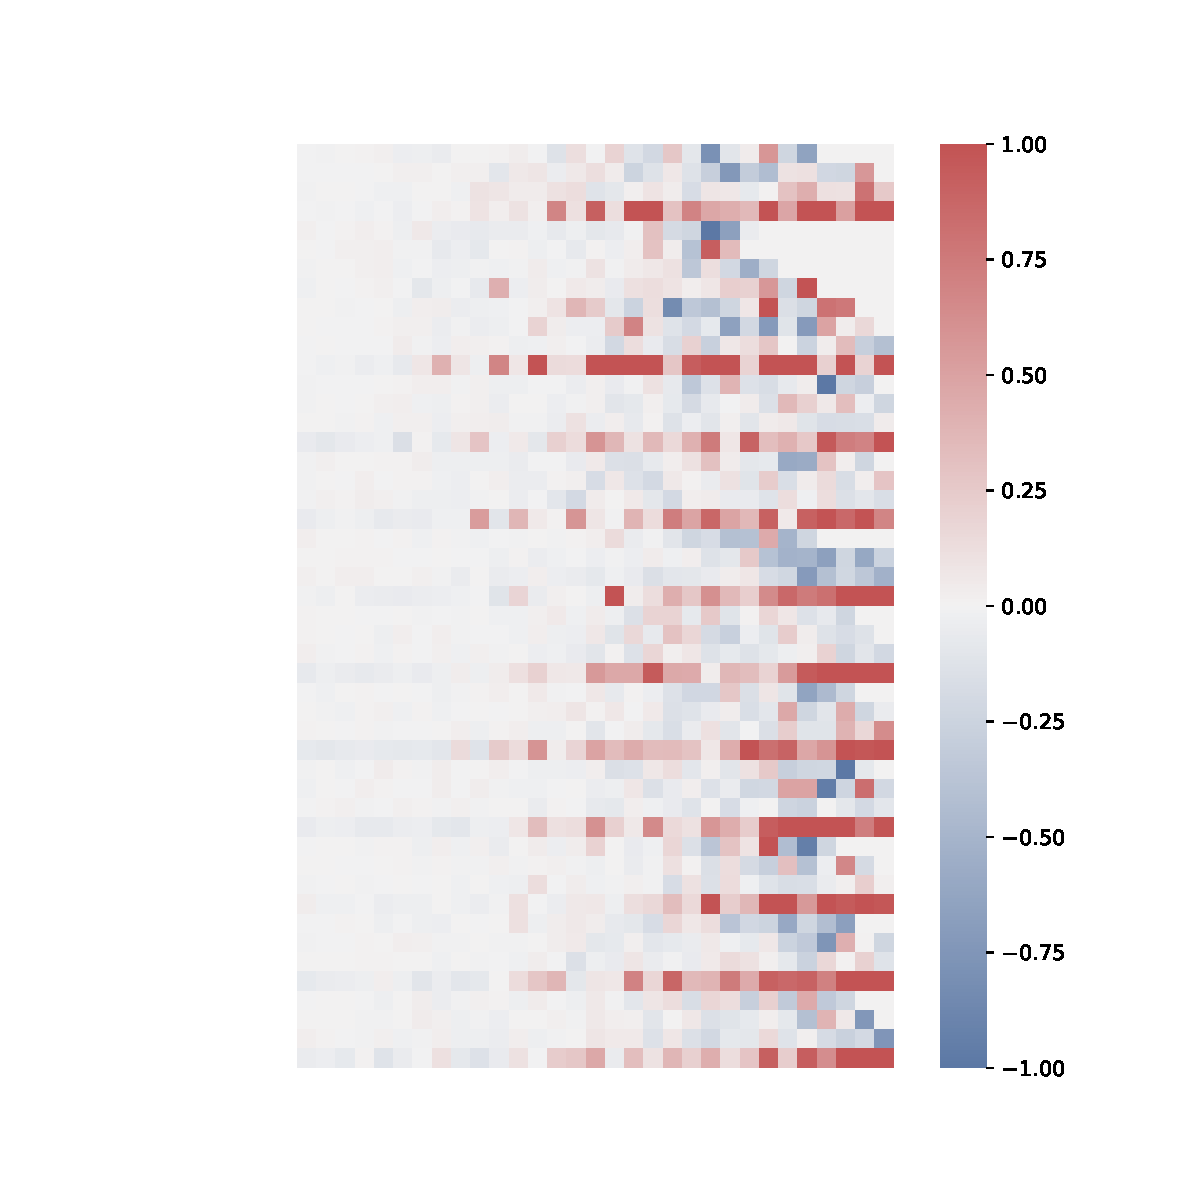
\includegraphics[width=4in]{figure/gene coef.pdf}
	\caption{基因对于拍卖成交价格的影响}
	\label{fig:gene coef}
\end{figure}

对于generation,其系数变化如图\ref{fig:generation coef}所示。可以看到从0代猫到3代猫之间价格迅速下降,从5代猫到15代猫之间猫的代数对于价格没有太大影响,15代以后又有小幅下降。

\begin{figure}[!htbp]
	\centering
	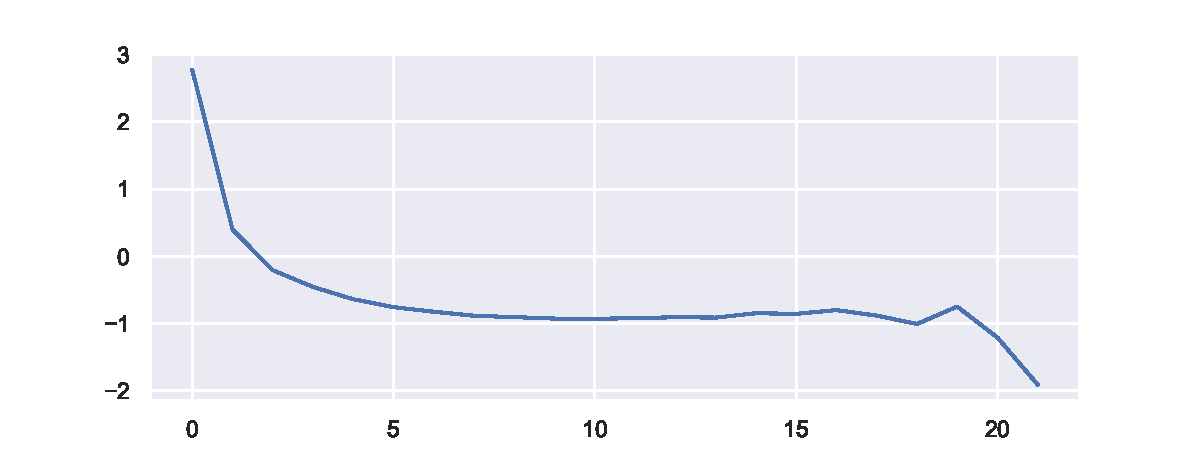
\includegraphics[width=4in]{figure/generation coef.pdf}
	\caption{代数对于拍卖成交价格的影响}
	\label{fig:generation coef}
\end{figure}

\section{总结与展望}
CryptoKitties是以太坊DApp的先驱者,但是近年来,CryptoKitties的市场活跃度在逐渐下降,市场价格先下降、后上升、再下降,市场目前需求量与供给量持平或大于供给量。CryptoKitties的大部分用户以收藏NFT为主要目的,少部分人以牟利为主要目的。用户在CryptoKitties的盈利模式为购入种猫、让自己的猫繁殖或购买生育权繁殖、将繁殖后出生的小猫或其它手中的猫再卖出去,以赢得利润。CryptoKitties市场中的交易价格受到多方面的因素影响。在猫本身方面,包括猫的基因、猫的代数、猫的生育次数等等。在市场方面,包括创建拍卖的次数、拍卖成功的次数、以太币价格等等。此外还受到时间等因素的影响。通过线性模型拟合2018年的数据,其$R^2$为0.703,可解释性较高。

线性模型需要基于一定的假设。若拍卖价格等变量没有进行对数化处理,则$R^2$仅有0.1左右,即使进行对数化处理,也仅仅假设该变量的对数满足线性化假设。然而在实际过程中,解释变量与被解释变量之间的关系可能远比指数更复杂。因此在未来,可以尝试加入交叉项或其它函数形式来丰富模型的假设,或者使用深度学习的方法,让模型学习更加复杂的特征。


\nocite{*}
\printbibliography[heading=bibintoc, title=参考文献]
\appendix
% \section*{附录}
% \section{代码}
% \subsection{网络自动化代码}
% \label{section:selenium code}
% \lstinputlisting[language=Python]{code/sql.py}



\end{document}